
\documentclass[times]{fldauth}

\usepackage{moreverb}

\usepackage[colorlinks,bookmarksopen,bookmarksnumbered,citecolor=red,urlcolor=red]{hyperref}

\newcommand\BibTeX{{\rmfamily B\kern-.05em \textsc{i\kern-.025em b}\kern-.08em T\kern-.1667em\lower.7ex\hbox{E}\kern-.125emX}}


\usepackage{graphicx}

\usepackage{epsfig}

\usepackage{comment}

\usepackage{epstopdf}


\usepackage{subfig}

\usepackage{bm}
\usepackage{hyperref,url}
\hypersetup{colorlinks=true, urlcolor=blue, linkcolor=blue, citecolor=red}

%\usepackage[obeyFinal]{todonotes}
\usepackage{todonotes}
\newcommand{\jrp}[1]{\todo[color=blue!30, size=\small]{JRP: #1}}
\newcommand{\JGnote}[1]{\fbox{\parbox{\textwidth}{ \color{blue} JG: #1}}}

\usepackage{amssymb,amsmath,array}

\newcommand{\frc}{\displaystyle\frac}
\newcommand{\PN}[2][error]{P$_{#1}$DG-P$_{#2}$}
\newcommand{\PNDG}[2][error]{P$_{#1}$DG-P$_{#2}$DG}

% Adding line numbers ... and colours for comments
\usepackage{lineno}
\linenumbers
\pagewiselinenumbers
\usepackage{color}
\newcommand{\red}{\textcolor{red}}
\newcommand{\blue}{\textcolor{blue}}


\begin{document}


\address{\affilnum{1} Novel Reservoir Modelling and Simulation Group, Department of Earth Science and Engineering, Imperial College London, UK. \\ \affilnum{2}Applied Modelling and Computation Group, Department of Earth Science and Engineering, Imperial College London, UK. \\ \affilnum{3} Environmental and Industrial Fluid Mechanics Group, School of Engineering, University of Aberdeen, UK.}
\corraddr{Novel Reservoir Modelling and Simulation Group, Department of Earth Science and Engineering, Imperial College London, UK. E-mail: dimitrios.pavlidis@imperial.ac.uk}

\runningheads{J. L. M. A. Gomes \textit{et al.}}{A Force-Balanced CVFEM for Multi-phase Porous Media Flow Modelling}

\title{A Force-Balanced Control Volume Finite Element Method for Multi-Phase Porous Media Flow Modelling}


\author{J. L. M. A. Gomes\affil{3,1}, D. Pavlidis\corrauth\affil{1,2}, P. Salinas\affil{1,2}, Z. Xie\affil{1,2}, J. R. Percival\affil{2}, \\Y. Melnikova\affil{1,2}, C. C. Pain\affil{1,2}, M. D. Jackson\affil{1}}


\begin{abstract}
  A novel method for simulating multi-phase flow in porous media is
  presented. The approach is based on a control volume finite element
  mixed formulation and new force-balanced finite element pairs. The
  novelty of the method lies in: (a) permitting both continuous and
  discontinuous description of pressure and saturation between
  elements; (b) the use of arbitrarily high-order polynomial
  representation for pressure and velocity and (c) the use of
  high-order flux-limited methods in space and time to avoid
  introducing non-physical oscillations while achieving high-order
  accuracy where and when possible. The model is initially validated
  for two-phase flow. Results are in good agreement with analytically
  obtained solutions and experimental results. The potential of this
  method is demonstrated by simulating flow in a realistic geometry
  composed of highly permeable meandering channels.
\end{abstract}

\keywords{CVFEM mixed formulation; Discontinuous Galerkin; Flux-limiting; High-order method; Multi-phase flows; Porous media flows}

\maketitle

\section{Introduction}

Numerical modelling of multi-phase flows in porous media has
applications in a wide range of disciplines, including hydrocarbon and
groundwater production, safety assessment of deep geological disposal
of radioactive waste, and carbon capture and storage \cite{chen_2006,
 aiea_1999,pruess_1990c,jiang_2011}. Such applications often
include complex geometries with irregular (and often internal)
boundaries between rock types with contrasting porosity and
permeability. Accurately capturing these complex geometries is a key
challenge when simulating such flows.

Finite difference methods (FDM) have been extensively used for
modelling fluid flows in porous media
\cite{aziz_1986, chen_1997, chen_2005}. However, they are strongly
dependent on mesh quality and orientation, and cannot easily represent
complex geometries. In addition, FDM can produce excessive numerical
dispersion in heterogeneous porous media flows \cite{chavent_1986}. 

The geometrical flexibility of finite element methods (FEM) has been
shown to overcome these deficiencies. Among FEM-based formulations for
porous media, the control volume finite element method (CVFEM) is
increasingly popular as it can guarantee local mass conservation, it
has the potential to be high-order accurate, and is able to use
tetrahedral, geometry-conforming elements \cite{forsyth_1990,
  cordazzo_2004, geiger_2004, hurtado_2007}. Huber and Helmig \cite{huber_2000}
demonstrated that the vertex-centred, finite volume-finite element
method (or Box scheme) can achieve similar goals (see also \cite{helmig_1997}).

Durlofsky \cite{durlofsky_1993,durlofsky_1994} compared the performance of a
mixed FEM formulation (piece-wise linear in velocity and piece-wise
constant in pressure) and the classical CVFEM for single phase Darcy
flows. It was concluded that the latter is computationally more
efficient and numerically more accurate than the former for problems
involving a (relatively) small number of degrees of freedom. Moreover,
for complex heterogeneous problems with sharp changes in material
properties, the mixed FEM formulation often led to physically
unrealistic solutions.  Cumming {\it et al.} \cite{cumming_2011} demonstrated that a
CVFEM-based discretisation could be used to solve the Richards
equation (coupled mass conservation and Darcy equations) in
heterogeneous porous media with relatively small computational
overhead, compared with traditional, coupled velocity-pressure based
formulations.  Mass balance was enforced as described by Kirkland {\it et al.}
\cite{kirkland_1992} (see also \cite{forsyth_1990,cumming_phd2012}). However, CVFEM often requires
high resolution meshes in regions where material properties vary
abruptly, such as permeability contrasts at (for example)
fracture-matrix interfaces, or boundaries between different rock
types. Control volume (CV) boundaries span finite elements where
material properties are defined; therefore, some average value of the
permeability must be calculated across CV interfaces. This often leads
to excessive numerical dispersion, especially in highly heterogeneous
media \cite{nick_2011b, nick_2011a}.

Discontinuity-capturing schemes (e.g. shock waves, contact
  surface or material discontinuities --
  see \cite{brooks_1982,tezduyar_1986}), were originally developed to
resolve sharp changes in solution fields such as velocity or
saturation. Related discontinuity-capturing schemes include the
discontinuous-Galerkin FEM (DGFEM) scheme in which continuity of the
solution is not explicitly enforced, allowing sharp changes in the
solution fields to be captured. The DGFEM scheme is stabilised,
locally conservative and designed to achieve high-order
accuracy. DGFEM solution fields are allowed to be discontinuous at the
element faces; thus, the solution is able to handle discontinuities in
material properties at internal boundaries. In addition, DGFEM is
well-suited to deal with interface problems by incorporating
specially-designed interface fluxes. These properties have attracted
the attention of the porous media flow community over the past 15
years (see \cite{riviere_2000,riviere_2002,bastian_2002}) and are
utilised here.

In this paper, a novel CVFEM formulation which is conservative and
consistent is presented. The continuity equations are embedded into
the pressure equation to enforce mass conservation and the exact force
balance. The \PN[n]{m}[DG] family of triangular and tetrahedral finite
element pairs is used to discretise velocity and pressure in
space. For this element type, the velocity field is represented by
$n^{\rm th}$-order polynomials that are discontinuous across elements,
while the pressure field is represented by $m^{\rm th}$-order
polynomials that may be continuous (termed P$_n$DG-P$_m$) or
discontinuous (termed P$_n$DG-P$_m$DG) across elements. Control
volumes are dual to the pressure mesh. The formulation employs an
implicit algorithm with respect to time that is less restrictive than
the implicit-pressure-explicit-saturation (IMPES) scheme often adopted
in porous media flow problems (e.g. see \cite{aziz_1986, geiger_2004}).

The method is demonstrated using two families of element pairs: the
\PN[n]{m} pair which can allow the velocity to exactly represent the
pressure gradients in the flow solution for homogeneous material
properties; and the \PNDG[n+1]{n} pair, which has similar properties
to the \PN[n]{n+1} element pair, but allows a representation in which
pressure, saturation and other solution variables are discontinuous
across finite element boundaries. This solves the long-standing
problem described above with respect to the use of traditional CVFEM
to capture sharp changes in material properties.

Results using this method in simple geometries have been previously
reported in the literature
(e.g. see \cite{jackson_2015,kaisu}). However, the method has not
been described in detail or thoroughly validated, and its potential has not been
explored. The remainder of this paper is organised as follows. The
governing equations and numerical methods employed to solve them are
introduced in Section~\ref{overlapping_method_section}. Model set-up
and results including comparison against reference data are given in
Sections~\ref{setup} and~\ref{res}, respectively. Finally, 
concluding remarks are presented in Section~\ref{conc}.




\section{Governing Equations and Numerical Formulation}
\label{overlapping_method_section}

\subsection{A novel representation of multi-phase Darcy flows}
Darcy's law for immiscible multi-phase flow may be written in the form:
\begin{equation}\label{e:darcy_eqn}
  \mathbf{q}_{\alpha} =
  -\frac{\mathcal{K}_{{r}_\alpha}\mathbf{K}}{\mu_{\alpha}}\left(
  \nabla p_{\alpha} - {\mathbf{s}_{u}}_{\alpha} \right),
\end{equation}
where $\mathbf{q}_{\alpha}$ is the $\alpha$-th phase Darcy velocity,
$\mathbf{K}$ is the absolute permeability tensor of the porous medium,
$\mathcal{K}_{{r}_\alpha}\left(S_{\alpha}\right)$ is the phase
relative permeability, which is a function of the phase saturation
$S_{\alpha}\left(\mathbf{r},t\right)$. $\mu_{\alpha}$, $p_{\alpha}$,
$\rho_{\alpha}$, and $\mathbf{s}_{{u}_\alpha}$ are the phase dynamic
viscosity, pressure, density and source term, which may include gravity and/or
capillarity, respectively. 

Introducing a saturation-weighted Darcy velocity defined as
$\mathbf{u}_\alpha= \mathbf{q}_\alpha/S_\alpha$, then
Eqn.~\ref{e:darcy_eqn} may be rewritten as:
\begin{equation}
  \mathbf{v}_\alpha={\underline {\underline \sigma}}_{\alpha}
  \mathbf{u}_{\alpha} = - \nabla p_{\alpha} +
         {\mathbf{s}_{u}}_{\alpha},
  \label{force-bal}
\end{equation}
where ${\underline {\underline \sigma}}_{\alpha}=\mu_\alpha S_\alpha
\left(\mathcal{K}_{{r}_\alpha}\mathbf{K}\right)^{-1}$ represents the
implicit linearisation of the viscous frictional forces. The force per
unit volume $\mathbf{v}_\alpha$, defined as ${\underline {\underline
    \sigma}}_{\alpha} \mathbf{u}_\alpha$, is used as a prognostic
variable in this approach, as explained in
Section~\ref{Section:Force_density}.

In order to discretise Eqn.~\ref{force-bal}, a finite element
representation for $\mathbf{v}_\alpha$ and $p$ is assumed, expressed
in terms of their FE basis functions $Q_{j}$ and $P_{j}$,
respectively, as:
\begin{equation}
  \mathbf{v}_\alpha(\bm{r},t) = \sum\limits_{j=1}^{\mathcal{N}_u}
  Q_{j}(\bm{r})\mathbf{v}_{\alpha,j}(t) \;\;\;\;\text{ and } \;\;\;\;
  p(\bm{r},t) = \sum\limits_{j=1}^{\mathcal{N}_p}
  P_{j}(\bm{r})p_{j}(t).
\end{equation} 
Here $\mathcal{N}_{u}$ and $\mathcal{N}_{p}$ are the total number of
degrees of freedom for the FE force and pressure representations. Each
component of the weak form of the force balance (Eqn.~\ref{force-bal})
is tested with the $\mathbf{v}_\alpha$ basis function space to obtain:
\begin{eqnarray}
  \sum\limits_{E} \left. \int\limits_{\Omega_E} { {Q}}_i \left (
             {\mathbf v}_\alpha + \nabla p  -\rho_\alpha g \mathbf{d} -{\mathbf s}_{u_\alpha}
             \right) dV \right. + \displaystyle \oint_{\Gamma_{E}}
                   {Q}_i {\mathbf n} \left(p - \tilde{p}\right)
                   d\Gamma + \nonumber \\ \oint_{\Gamma_{\Omega}} {
                     Q}_i {\mathbf n} \left(p - p_\text{bc}\right) d\Gamma
                   = \bm{0},
                   \label{force-semi-disc} 
\end{eqnarray} 
\red{DP, shouldn't this equation be 
\begin{eqnarray}
  \sum\limits_{E} \left. \int\limits_{\Omega_E} { {Q}}_i \left (
             {\mathbf v}_\alpha + \nabla p  -{\mathbf s}_{u_\alpha}
             \right) dV \right. + \displaystyle \oint_{\Gamma_{E}}
                   {Q}_i {\mathbf n} \left(p - \tilde{p}\right)
                   d\Gamma + \nonumber \\ \oint_{\Gamma_{\Omega}} {
                     Q}_i {\mathbf n} \left(p - p_\text{bc}\right) d\Gamma
                   = \bm{0},\nonumber
                   \label{force-semi-disc} 
\end{eqnarray} 
instead (to be consistent w Eqn. 3)? }

where $\Omega_E$ and $\Gamma_{E}$ are the volume and boundary of
element $E$, respectively, and $\Gamma_{\Omega}$ is the boundary of
the computational domain. The numerical pressure $\tilde{p}$ appearing
in the jump condition (second term in Eqn.~\ref{force-semi-disc}) is
the arithmetic mean of the potentially discontinuous pressure across
the element $E$. This term vanishes when a continuous formulation is
used to discretise the pressure field. The last term in
Eqn.~\ref{force-semi-disc} is used to weakly enforce the pressure
level to $p_\text{bc}$ on a computational domain boundary.

In matrix form, Eqn.~\ref{force-semi-disc} is:
\begin{equation}
  {\mathbf M} \underline {\mathbf v} = -{\mathbf C} \underline
  {\mathbf p} + \underline {\mathbf
    s}_{u}, \label{force-balance-matrix-form}
\end{equation}
where $\underline{\bf v}$ and $\underline{\bf p}$ solution-vectors are
defined as:
\begin{eqnarray}
  &&\underline{{\bf v}} = \left( 
  \left( {v_x},{v_y},{v_z} \right)  _{1,1},
  \left( {v_x},{v_y},{v_z} \right)  _{2,1},\ldots,
  \left( {v_x},{v_y},{v_z} \right)  _{\mathcal{N}_\alpha,\mathcal{N}_u}
  \right)^{T}
  \;\text{and} \nonumber \\ &&
  \underline{{\bf p}} = \left(p_1, p_2, p_3, ...,
  p_{\mathcal{N}_p}\right)^T. \nonumber \nonumber
\end{eqnarray}
$\mathcal{N}_{\alpha}$ is the number of phases and $v_x$, $v_y$ and
$v_z$ are the components associated with the $x$, $y$ and $z$
dimensions, respectively. Finally, the mass matrix ${\mathbf M}$,
gradient matrix ${\mathbf C}$ and source vector $\underline {\mathbf
  s}_{u}$ are defined as:
\begin{eqnarray}
  && \left[{\mathbf M}^{(i,j)}\right]_{k,l} = \int_{\Omega} Q_{k}
  \left[\underline{\underline{\sigma}}_{\alpha}\right]_{i,j} {Q}_{l}
  dV, \nonumber \\ && {\left[\bm{C}^{(i,i)}\right]_{k,l} =
    \int_{\Omega} Q_{k} \frac{\partial P_{l}}{\partial r_i} dV -
    \oint_{\Gamma_{E}} \displaystyle\frac{1}{2} Q_{k} n_i^{(E,l)}
    P_{l} d\Gamma - \oint_{\Gamma_{\Omega}} \displaystyle Q_{k} n_i
    P_{l} d\Gamma}, \nonumber \\ &&
  {\left[\bm{s}_{u}^{(i,i)}\right]_{k} = \int_{\Omega} Q_k}
  \left[{\mathbf s}_{u_\alpha} \right]_i dV -
  \oint_{\Gamma_{\Omega}}\displaystyle Q_{k} n_i p_\text{bc} d\Gamma,
  \nonumber
\end{eqnarray}
where $i$ and $j$ are dimensions and $k$ and $l$ are the degrees of
freedom of element $E$. Here, $\bm{n} = \left(n_{1}, n_{2},
n_{3}\right)^{T}$ is the outward-pointing normal vector of the domain
$\Omega$. $\bm{n}^{(E,l)}$ is the normal to the boundary of element
$E$ and is outward-pointing if $P_{l}$ takes support on $E$, and
inward-pointing otherwise.

The saturations are computed in CV space, whereas the permeability
tensor $\left(\mathbf{K}\right)$ is assumed piece-wise constant in FE
space. Thus the viscous-friction damping tensor $ {\underline
  {\underline \sigma}}_{\alpha}$ is piece-wise constant within the
sub-control volumes defined through intersections between the elements
and control volumes (see Fig.~\ref{fem_cv_represent_a}).



\subsection{Control volume finite element types}
In the formulation presented here, pressure, velocity, permeability and porosity are represented FE-wise, however saturation, relative permeability and fluid properties such as viscosity and density are represented CV-wise. Figure~\ref{fem_cv_represent_a} displays the two families of element types presented in this paper: Fig.~\ref{fem_cv_represent_a} (a) shows the P$_{n}$DG-P$_{n+1}$ element type, with $n = 1$, in two dimensions (2D). Here, the velocity field is linear and discontinuous (between elements) whilst pressure has a quadratic and continuous (between elements) representation with the CV's span various elements. Figure~\ref{fem_cv_represent_a} (b) shows the P$_{n+1}$DG-P$_{n}$DG element type, with $n = 1$ (also in 2D). Here, the velocity field is quadratic and discontinuous (between elements) whereas pressure has a linear and discontinuous (between elements) representation and the CV's do not span elements.

\begin{figure}[h!]
\subfloat[P$_1$DG-P$_2$]{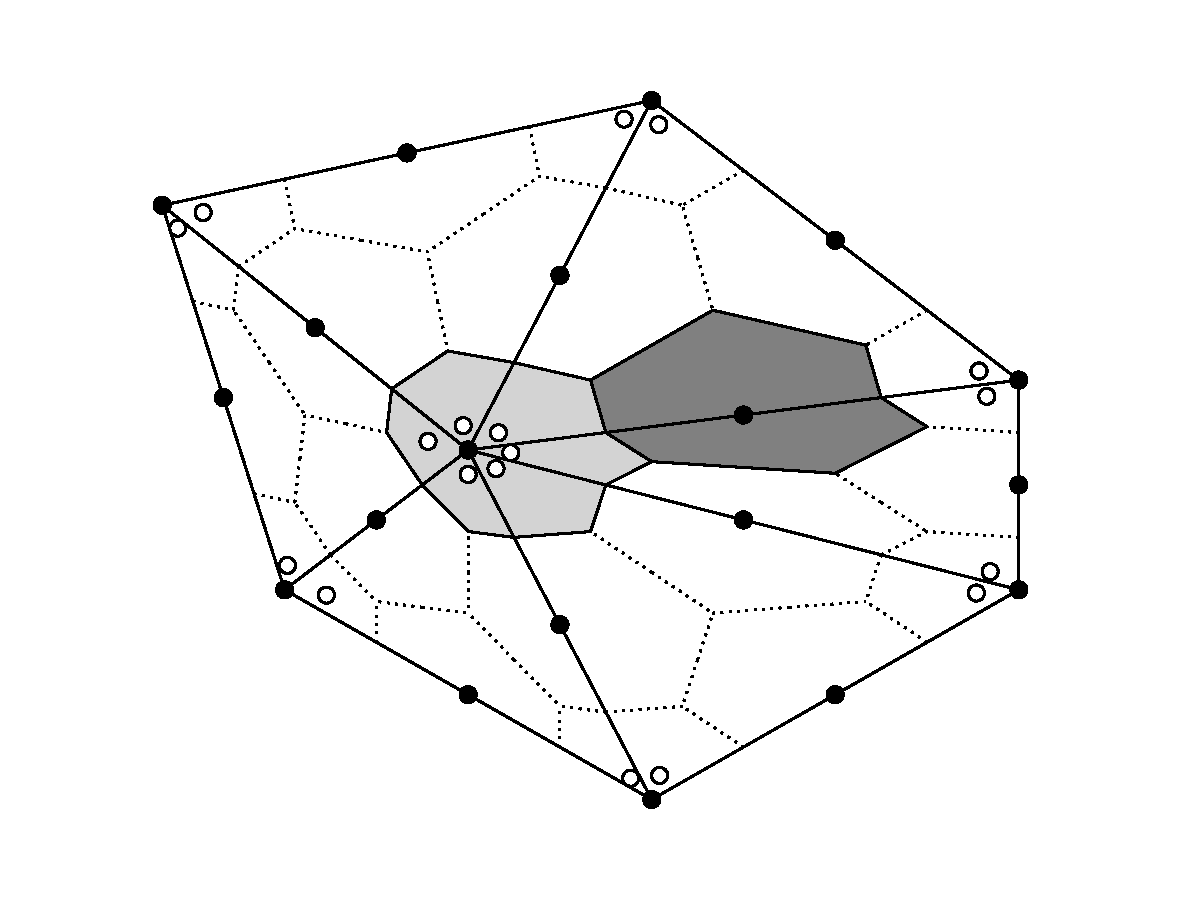
\includegraphics[width=.5\textwidth]{p1dgp2-cont-sat.pdf}}
\subfloat[P$_2$DG-P$_1$DG]{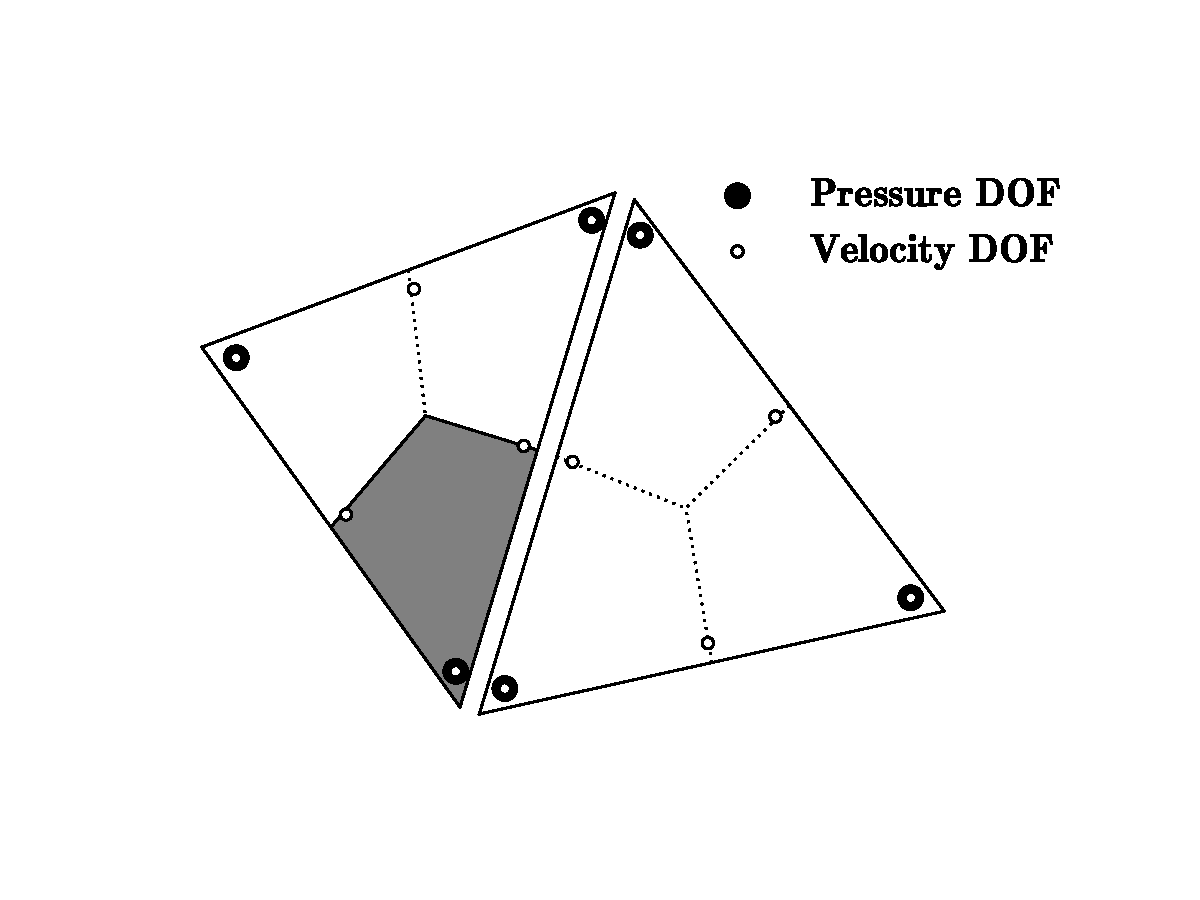
\includegraphics[width=.5\textwidth]{p2dgp1-dg-sat.pdf}}
\caption{2D representation of the element pairs presented in this work. Shaded areas denote control volumes (in which saturation is   stored), black points represent the pressure nodes and white points the velocity nodes. Note that in (b) velocity and pressure nodes overlap in the triangles' vertices.}
    \label{fem_cv_represent_a}
\end{figure} 

\subsection{Finite element representation of velocity} \label{Section:Force_density}
From Eqn.~\ref{e:darcy_eqn}, it can be seen that the velocity field depends, among other fields, on the absolute permeability which is FE-wise, and the relative permeability which is CV-wise. This means that the velocity representation is different in each CV. However, the quantity $\mathbf{v}_\alpha$ is homogeneous within an element and this is stored using FE representation. To obtain the velocity $\mathbf{u}_{\alpha}$ in a particular CV within a FE, Eqn.~\ref{force-bal} is used.


\subsection{Saturation and global mass conservative equations} \label{Section:Saturation_Global}
Here, the saturation conservation equations are discretised and the
global mass balance equation is derived. In this work, fluids are
assumed incompressible. The saturation equation can be written as:
\begin{equation}
  \phi\displaystyle\frac{\partial S_{\alpha} }{\partial t} + \nabla
  \cdot \left( {\mathbf u}_{\alpha} S_{\alpha}\right) =
  s_{cty,\alpha},
  \label{saturation_equation}
\end{equation}
where $\phi$ is the porosity and $s_{cty}$ is a source
term. Eqn.~\ref{saturation_equation} is discretised in space by
testing with CV basis functions $M_{i}$ and with the $\theta$-method
in time:
\begin{eqnarray}
  \int_{\Omega} M_{i} \displaystyle\frac{\phi \left({S_{\alpha
        i}^{n+1}}-{S_{\alpha i}^{n}}\right)}{\Delta t} dV + \nonumber
  \\ \oint_{\Gamma_{CV_{i}}} \left[\theta^{n+\frac{1}{2}} {\mathbf n}
    \cdot {\mathbf u}_{\alpha}^{n+1} S_{\alpha}^{n+1} +
    \left(1-\theta^{n+\frac{1}{2}}\right) {\mathbf n} \cdot {\mathbf
      u}_{\alpha}^{n} S_{\alpha}^{n} \right]d\Gamma = \int_{\Omega}
  M_{i} {s_{cty,\alpha}^{n+\theta}} dV,
  \label{detail-sat-eqn-k}
\end{eqnarray}
where $\mathbf{n}$ is the outward-pointing unit normal vector to the
surface ($\Gamma_{CV_{i}}$) of the control volume $i$ and $n$ is the
current time level. More details on the numerical methods used to
solve Eqn.~\ref{detail-sat-eqn-k} can be found in
\cite{pavlidis_2013b}.

The global continuity equation is obtained by summing
Eqn.~\ref{detail-sat-eqn-k} over all phases:
\begin{eqnarray}
  \sum\limits_{\alpha=1}^{\mathcal{N}_{\alpha}} \left\lbrace
  \int_{\Omega} M_{i} \displaystyle\frac{\phi\left({S_{\alpha
        i}^{n+1}}-{S_{\alpha i}^{n}}\right) } {\Delta t} dV +
  \right. \nonumber \\ \left. \displaystyle\oint_{{\Gamma_{CV}}_{i}}
  \left[\theta^{n+\frac{1}{2}} {\mathbf n} \cdot {\mathbf
      u}_{\alpha}^{n+1} S_{\alpha}^{n+1} +
    \left(1-\theta^{n+\frac{1}{2}}\right) {\mathbf n} \cdot {\mathbf
      u}_{\alpha}^{n} S_{\alpha}^{n} \right] \,d\Gamma -
  \right. \nonumber \\ \left. \displaystyle\int_{\Omega} M_{i}
  s_{cty,\alpha}^{n+\theta}\, dV \right\rbrace = 0.
           \label{detail-sat-eqn-k-sum}
\end{eqnarray}
Eq.~\ref{detail-sat-eqn-k-sum} is also bounded by the constraint:
\begin{equation}
  \sum\limits_{\alpha=1}^{\mathcal{N}_{\alpha}} {S_{\alpha}^{n}}_{i} =
  1, \quad \forall n.
\end{equation}
Solving for ${\mathbf u}^{n+1}$ in matrix form,
Eqn.~\ref{detail-sat-eqn-k-sum} becomes:
\begin{equation}
  {\mathbf B}^T \underline{\bf v}^{n+1} = \underline{\bf s}_{p}.
  \label{glob-cty-matrix}
\end{equation}


\subsection{Velocity at control volume interfaces} \label{opt-up} 
The velocity to be used at the interface between CV's in the saturation conservation (Eqn.~\ref{detail-sat-eqn-k}) and global continuity (Eqn.~\ref{detail-sat-eqn-k-sum}) equations needs to be determined. On the CV faces, there is no information about the flow direction as the velocity is discontinuous at the CV boundaries. The discontinuities occur between (a) control volumes within each FE and (b) between elements when using the \PNDG[n+1]{n} element pair.

In order to calculate the velocity across CV's within a FE, an average velocity at the interface of control volumes {\it i} and {\it j} is defined as:
\begin{equation}
  {\tilde{\bf u}}_\alpha = \frac{1}{2} \left[ {{\bf u}_\alpha}_i + {{\bf u}_\alpha}_j \right].
\end{equation} 
From this, the interface velocities at either side of the interface can be obtained from:
%\begin{equation}
%  {\tilde{\bf u}}_{\alpha k} = \underline{\underline{\sigma}}_{\alpha
%    k}^{-1}{\tilde{{\bf u}}}_{\alpha}, \;\;\;\; k=\{i,j\}.
%  \label{two-vels}
%\end{equation} 
\begin{equation}
  {\tilde{\bf u}}_{\alpha k} = \underline{\underline{\sigma}}_{\alpha k}^{-1}{{\bf \tilde{v}}}_{\alpha}, \;\;\;\; k=\{i,j\}. 
  \label{two-vels}
\end{equation} 

These velocities have the same direction and differ only in magnitude, so using them to define an upwind direction is not ambiguous. If an upwind method for calculating the interface velocity is applied then,
\begin{equation}
  {\tilde{\bf u}}_{\alpha} = \tilde{\bf u}_{\alpha k},\label{interface_velocity_upwind}
\end{equation}
where $k=i$ if ${\bf n}\cdot{\bf u}_{\alpha}>0$ (CV {\it i} outgoing information), and $k=j$ if ${\bf n}\cdot{\bf u}_{\alpha}<0$ (CV {\it i} incoming information). 

However, upwind methods yield dissipative solutions therefore, in order to obtain a high-order approximation of the velocity at the interface, the saturation at the interface $\tilde{S}_{\alpha}$ is calculated using a finite element representation of the saturation following the upwind direction. $\tilde \sigma_{\alpha}$ can then be calculated using second-order Taylor series:
%\begin{small}
\begin{equation}
  \underline{\underline{\tilde{\sigma}}}_{\alpha} =
  \underline{\underline{\sigma}}_{\alpha k} +
  \left(\tilde{S}_{\alpha}-S_{\alpha k}\right) \left(\frc{\partial
    \underline{\underline{\sigma}}_{\alpha}}{\partial
    S_{\alpha}}\right)_{k} +
  \frc{1}{2}\left(\tilde{S}_{\alpha}-S_{\alpha k}\right)^{2} \left[
    \frc{ \left(\frc{\partial
        \underline{\underline{\sigma}}_{\alpha}}{\partial
        S_{\alpha}}\right)_{k} - \left(\frc{\partial
        \underline{\underline{\sigma}}_{\alpha}}{\partial
        S_{\alpha}}\right)_{l} } { \left(S_{\alpha k}-S_{\alpha
        l}\right) } \right],
  \label{sigma-out}
\end{equation}
%\end{small}
where $k=i$ and $l=j$ if ${\bf n}\cdot{\bf u}_{\alpha}>0$ and, $k=j$ and $l=i$ if ${\bf n}\cdot{\bf u}_{\alpha}<0$. Therefore, the final interface velocity (Eqn.~\ref{interface_velocity_upwind}) can be obtained from:
%\begin{equation}
%  {\tilde{\bf u}_{\alpha}} = \underline{\underline{\tilde{\sigma}}}_{\alpha}^{-1} \left[\displaystyle\frac{1}{2} \left( {{\bf u}_\alpha}_i + {{\bf u}_\alpha}_j \right)\right], \label{mean_int_vel}  
%\end{equation} 
\begin{equation}
  {\tilde{\bf u}_{\alpha}} = \underline{\underline{\tilde{\sigma}}}_{\alpha}^{-1} \left[\displaystyle\frac{1}{2} \left( {{\bf v}_\alpha}_i + {{\bf v}_\alpha}_j \right)\right], \label{mean_int_vel}  
\end{equation} 
%The interface velocity obtained from Eqn.~\ref{mean_int_vel} is bounded to ensure that its normal component ${\tilde{\bf u}_\alpha}\cdot {\bf n}$ lies between ${\tilde{\bf u}_{\alpha i}}\cdot {\bf n}$ and ${\tilde{\bf u}_{\alpha j}}\cdot {\bf n}$. The result of this is also bounded between the velocities ${{\bf u}_\alpha}_i\cdot {\bf n}$ and ${{\bf u}_\alpha}_j\cdot {\bf n}$.
The interface velocity obtained from Eqn.~\ref{mean_int_vel} is bounded to ensure that its normal component ${\tilde{\bf u}_\alpha}\cdot {\bf n}$ lies between ${\tilde{\bf u}_{\alpha i}}\cdot {\bf n}$ and ${\tilde{\bf u}_{\alpha j}}\cdot {\bf n}$. The result of this is also bounded between the velocities ${{\bf v}_\alpha}_i\cdot {\bf n}$ and ${{\bf v}_\alpha}_j\cdot {\bf n}$.

\medskip

In a fully discontinuous formulation with \PNDG[n+1]{n} element pairs, the interface velocity (now between neighbour elements) can not be calculated using Eqn.~\ref{mean_int_vel} due the elliptic nature of the discretised non-symmetric pressure equation, Eqn.~\ref{force-balance-matrix-form}. This means that information is propagated in all directions across the (discontinuous) domain and hence, taking the upwind velocity as commonly done within an element is not an adequate strategy.
 
For two neighbouring CV's $i$ and $j$ with common FE interface ({\it e.g.}, see Fig.~\ref{fem_cv_represent_a}b for \PNDG[2]{1} element pair), $\tilde{\bf u}_\alpha$ can be calculated by using a volume-weighted harmonic mean. However, the volume $\mathcal{V}$ of the control volume and $\underline{\underline{\sigma}}_{\alpha}$ act on the velocity in a very similar way. Hence, the velocity at the interface is expressed as,
\begin{equation} 
  {\tilde{\bf u}_\alpha} =  \left(\mathcal{V}_{j}  
    \underline{\underline{\sigma}}_{\alpha j} \, {\bf
      u}_{\alpha i} + \mathcal{V}_{i} \underline{\underline{\sigma}}_{\alpha i}\, {\bf
      u}_{\alpha j} \right) \left(  \mathcal{V}_{i} 
    \underline{\underline{\sigma}}_{\alpha i} +
    \mathcal{V}_{j} 
    \underline{\underline{\sigma}}_{\alpha j} \right)^{-1}.
\end{equation} 


\subsection{Weak enforcement of boundary conditions}\label{bcs-rel-perm} 
Suitable boundary conditions for velocity can be applied by the
discontinuous formulation above as well as by the upwinding in the
continuous formulation. In fact, exactly the same boundary condition
implementations, as used in the discontinuous formulation, can be
applied across the boundaries of the domain by taking information from
`just outside' the domain rather than from the neighbouring elements.

Saturation boundary conditions are relatively straightforward. One
typically takes the saturation from `just outside' the domain
($S_{\alpha, \text{bc}}$) and the flux becomes $\left({\bf n}\cdot
{\bf u}_{\alpha}\right)S_{\alpha,\text{bc}}$, if ${\bf n}\cdot {\bf
  u}_{\alpha} < 0$. If the velocity is also specified (${\bf
  u}_{\alpha,\text{bc}}$) then this becomes part of the incoming flux
$\left({\bf n}\cdot {\bf
  u}_{\alpha,\text{bc}}\right)S_{\alpha,\text{bc}}$.

In case of specified pressure for outflow boundaries
$\left(\right.{\bf n}\cdot {\bf u}_\alpha>0\left.\right)$ the flux is
${\bf n}\cdot {\bf u}_\alpha {S_\alpha}$, in which neither ${\bf
  u}_\alpha$ nor ${S_\alpha}$ are specified.

However, for inflow boundaries with specified pressure
$\left(\right.{\bf n}\cdot {\bf u}_\alpha<0\left.\right)$ the flux is
${\bf n}\cdot {\bf u}_{\alpha,\text{bc}} S_{\alpha,\text{bc}}$, in
which ${\bf u}_{\alpha,\text{bc}}$ is calculated using:
\begin{equation}
  {\bf u}_{\alpha,\text{bc}} = 
    \underline{\underline{\sigma}}_{\alpha,\text{bc}} ^{-1}
    \underline{\underline{\sigma}}_{\alpha}  
              {\bf u}_{\alpha},
\end{equation}
where $\underline{\underline{\sigma}}_{\alpha,\text{bc}}$ is
calculated using $S_{\alpha,\text{bc}}$.

It should be noted that this flux condition must be used in both the
discretised saturation and global continuity equations, since the
latter is a summation of the former. The specified pressure condition
becomes a surface flux condition in the force balance equation
(Eqn.~\ref{force-semi-disc}), which effectively relaxes the pressure
$p$ to its face value counterpart $p_\text{bc}$ at the boundaries.


\subsection{Solving the linear equations}\label{Section:SolvingLinearEqns}
The global mass balance equation (Eqn.~\ref{glob-cty-matrix}) and
force balance equations (Eqn.~\ref{force-balance-matrix-form}) are
solved by substituting $\underline{\mathbf v}$ and solving the system
of equations for pressure. At time level $n+1$,
Eqns.~\ref{force-balance-matrix-form} and ~\ref{glob-cty-matrix} can
be rewritten as:
\begin{displaymath}
  \begin{cases}
    \mathbf{M} \underline{\bf v}^{n+1} = \mathbf{C}\underline{\bf
      p}^{n+1} + \underline{\bf s}_{u}^{n+1} \\ \mathbf{B}^{T}
    \underline{\bf v}^{n+1} = \underline{\bf s}_{p}^{n+1},
  \end{cases}
\end{displaymath}
respectively. Application of a discontinuous FEM for
$\mathbf{v}$ leads to a block-diagonal $\mathbf{M}$ matrix that
can be readily inverted, each block being local to an
element. Multiplying Eqn.~\ref{force-balance-matrix-form} by
$\mathbf{B}^{T}\mathbf{M}^{-1}$ and summing up with
Eqn.~\ref{glob-cty-matrix}, $\underline{\mathbf v}^{n+1}$
vanishes and the pressure equation is obtained:
\begin{equation}
  \mathbf{B}^{T}\mathbf{M}^{-1} \mathbf{C} \underline{\bf p}^{n+1} =
  \underline{\bf s}_{p}^{n+1} - \mathbf{B}^{T} \mathbf{M}^{-1}
  \underline{\bf s}_{u}^{n+1}.
  \label{final_projection}
\end{equation}
Eqn.~\ref{final_projection} is solved for pressure and then the
velocity is obtained via Eqn.~\ref{force-balance-matrix-form}. The
computationally demanding effort to solve the pressure matrix equation
arising from the fully discontinuous FEM formulation is achieved using
a multigrid-like approach (see \cite{Brandt}). In this case the
`fine' mesh is the one obtained by the discontinuous system, whereas
the `coarse' mesh is obtained by creating a continuous system (from
the discontinuous system) by collapsing the pressure nodes. As in
multigrid, the coarse mesh solution is used to accelerate the
convergence of the fine mesh solution by calculating the error of the
current approximation.





\section{Model set-up}\label{setup}
The numerical model is evaluated using four two-phase flow test-cases (Sections~\ref{classical_BL}-~\ref{res5}). The modified Brooks-Corey model \cite{Alpak_1999,brooks_1964}: 
%\begin{eqnarray}
%k_{rw}\left ( S_{w} \right ) &=& \left ( \frac{S_w-S_{wirr}}{1-S_{wirr}-S_{nwr}} \right )^{n_w}, \\
%k_{rw}\left ( S_{w} \right ) &=& \left ( \frac{S_{nw}-S_{nwr}}{1-S_{wirr}-S_{nwr}} \right)^{n_{nw}}, 
%\end{eqnarray}
\begin{eqnarray}
   k_{rw}\left ( S_{w} \right ) &=& k_{rw}^{\circ} \left ( \frac{S_w-S_{wirr}}{1-S_{wirr}-S_{nwr}} \right )^{n_w}, \\
   k_{rnw}\left ( S_{w} \right ) &=& k_{rnw}^{\circ} \left ( \frac{S_{nw}-S_{nwr}}{1-S_{wirr}-S_{nwr}} \right)^{n_{nw}}, 
\end{eqnarray}
where subscripts {\it w} and {\it nw} indicate wetting and non-wetting phase. $k_{rw}^{\circ}$ and $k_{rnw}^{\circ}$ are end-point relative permeability to wetting and non-weting phases, $S_w$ and $S_{nw}$ are the wetting and non-wetting phase volume fractions, respectively. The exponents $n_w$ and $n_{nw}$ are both set to 2 for all test cases.

The length of all computational domains is 1 non-dimensional length
unit. Computational domain height, boundary conditions, exponents for
the wetting $n_w$ and non-wetting $n_{nw}$ phases in the Brooks-Corey
model, along with the irreducible wetting phase saturation $S_{wirr}$,
residual non-wetting phase saturation $S_{nwr}$ and mobility $M^0$ for
each test case are shown in Table~\ref{tab:1}.

\begin{table}[h!]
  \centering
  \small{
    \caption{Model set-up for test cases \ref{classical_BL} --
      \ref{res5}.\label{tab:1}}
    \begin{tabular}{c c c c c c c c c c c c c c c} 
      \hline
      & $M^0$ & $\phi$ & $\mathbf{K}_\text{1}$ & $\mathbf{K}_\text{2}$ & $\mathbf{K}_\text{3}$ & $S_{wirr}$ & $S_{nwr}$ & $u_{\mathrm{in}}$ & $\Delta p$ & height \\ \hline
      \ref{classical_BL} & 10 & 0.2 & 1.0 & N/A    & N/A & 0.2   & 0.3 & 0.2 & N/A & N/A\\
      \ref{res2}         & 10 & 0.4 & 1.0 & 2.5    & N/A & 0.1   & 0.2 & 1.0 & N/A & 1.0\\ 
      \ref{res4}         & 10 & 0.5 & 1.0 & 10$^2$ & N/A & 0.0   & 0.0 & N/A & 1.0 & 0.1\\
      \ref{res5}         & 4  & 0.2 & 1.0 & 2.0    & 10  & 0.2   & 0.2 & N/A & 1.0 & 0.1\\ \hline
    \end{tabular}
  }
\end{table}

In all test cases, the domain is initially saturated with the
non-wetting phase at $(1- S_{wirr}).$ The wetting phase is then
injected through the left boundary, displacing the non-wetting phase
towards the opposite boundary. The wetting phase is injected at a
uniform, constant velocity ($u_{\mathrm{in}}$) from the left boundary
for test cases  \ref{classical_BL} and  \ref{res2}. In test case \ref{res2} the
inlet velocity is weighted by the permeability. For test cases  \ref{res4} and  \ref{res5},
the flow is driven by a pressure difference ($\Delta p$)
between the inflow (left) and outflow (right) boundaries of the
computational domain. The pressure level at the outflow boundary is
set to 0 for all test cases.

For the test-cases considered here, porosity $\phi$ is assumed uniform and, for \ref{classical_BL} $\mathbf{K}$ is also uniform. However, for test-cases~\ref{res2}-~\ref{res5}, $\mathbf{K}$ is non-uniform and regions of constant $\mathbf{K}$ are used (subscript denotes region identities -- Figs.~\ref{fig:4reg_BL_schematic} and~\ref{fig:wedge_permeability}). For all cases $\mathbf{K}$ is assumed isotropic.

In Section~\ref{res}, four sets of numerical simulations are performed using the formulation introduced in Section~\ref{overlapping_method_section}.  The main aims of these simulations (Table~\ref{Table:SummaryTestCases}) are: a) to assess numerical convergence and accuracy; b) to validate the model against analytical (quantitative) and lab-experiments (qualitative) solutions; c) to numerically investigate the performance of \PN[1]{2} and \PNDG[2]{1} element-pairs in multiphase flows behaviour in highly heterogeneous media ({\it i.e.}, large permeability gradient) and; d) \red{any comment on test 4?} 
\begin{center}
\begin{table}[h]
    \caption{Summary of the test-cases performed in Section~\ref{res}}\label{Table:SummaryTestCases}
\begin{tabular}{c|l c l}
{\bf Test-Case} & {\bf Element-pairs}     & {\bf Dimensionality}   &   {\bf Main Features} \\
                &                         & {\bf and mesh}         &                  \\ 
\hline
4.1 (Buckley-   & \PN[1]{1},              &  2D and 3D             & Assessment of model  \\
Leverett)       & \PN[1]{2} and           &(structured/            & accuracy against analytical \\ 
                & \PNDG[2]{1}             & unstructured)          & solutions \\
\hline
4.2 (Immiscible &\PN[1]{2} and            &  2D                    &  Qualitative analysis of the \\
displacement)   &\PNDG[2]{1}              &(coarse and fine)       & model against lab-experiments\\
\hline
4.3 (Permeability &\PN[1]{2} and          & 2D                    & Numerical dispersion in \\
constrast and aspect ratio) &\PNDG[2]{1}  &(coarse and fine)      & high-permeability contrast. \\
\hline 
4.4 (Channelisation)& \PNDG[1]{1}          & 3D                    &  \red{?}            \\
                    & and \PNDG[2]{1}      &                       &                     \\
\hline 
\end{tabular}
\end{table}
\end{center}


%%%
%%%
%%%
\section{Results}\label{res}



\subsection{The Buckley-Leverett test case}\label{classical_BL}

The Buckley-Leverett problem (non-wetting phase displaced by a wetting phase~\cite{buckley1942}) is simulated here. Despite the 1D nature of the problem, 2D and 3D simulations are performed to evaluate the multi-dimensional capabilities of the model (see Fig.~\ref{fig:maps2d_3d}). The \PN[1]{1}, \PN[1]{2} and \PN[2]{1}DG element pairs are used for these simulations.

\begin{figure}[h!]
  \begin{center}
    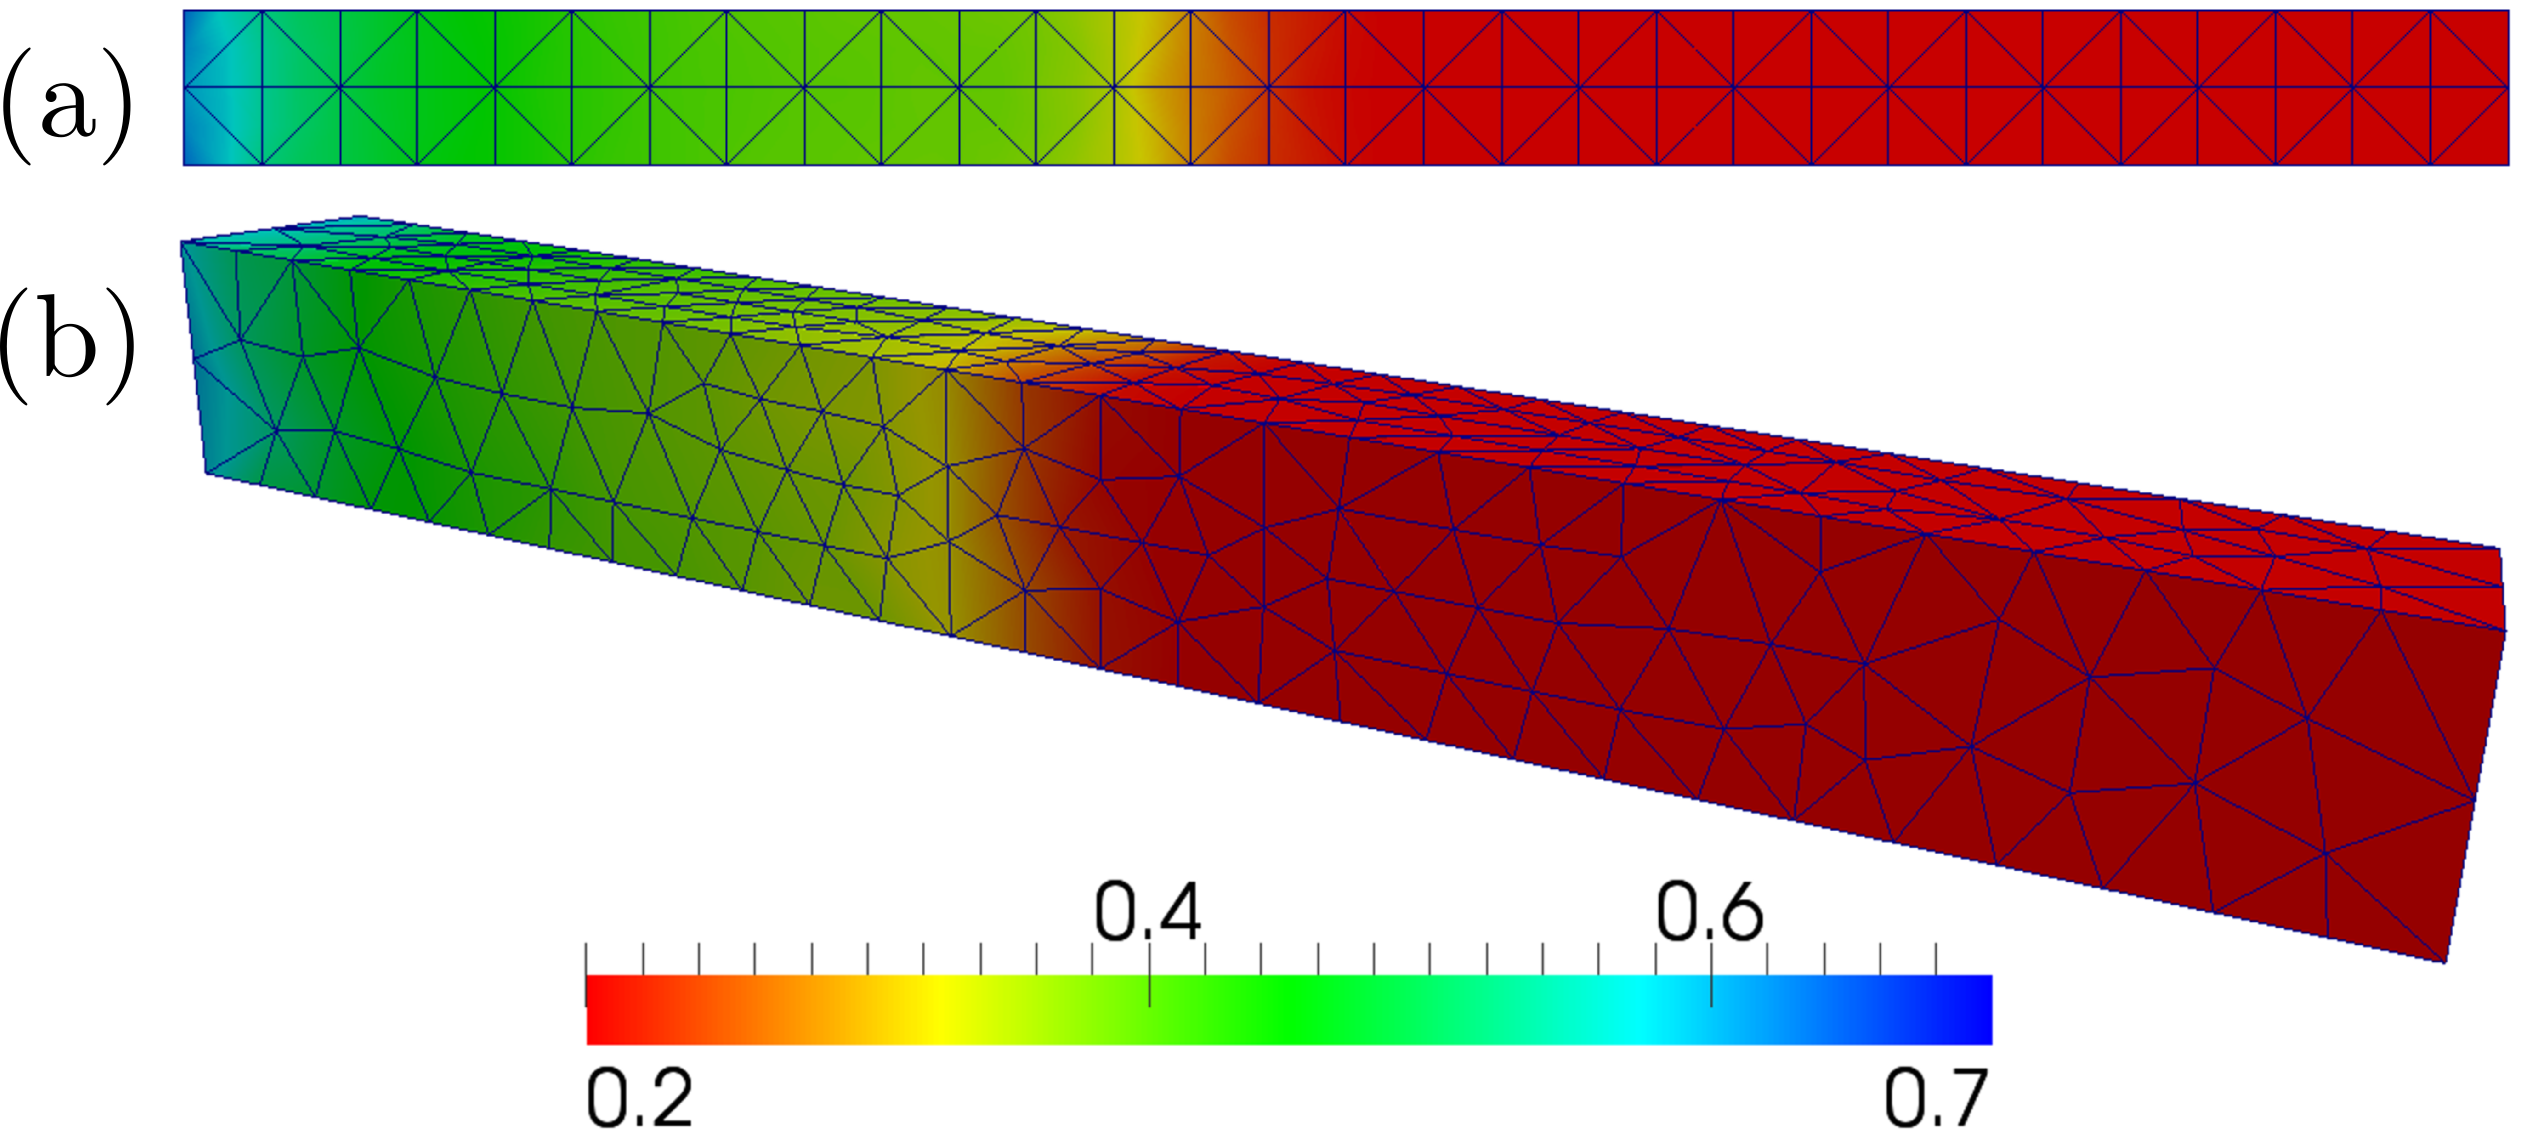
\includegraphics[width=0.75\textwidth]{BL_3D_merged}
    \caption{Wetting phase volume fraction for the Buckley-Leverett
      test case using the \PN[1]{2} element pair in 2D (a) and 3D
      (b). \label{fig:maps2d_3d}}
  \end{center}
\end{figure}

Figures~\ref{fig:BL_tests} (a-c) show phase volume fraction profiles of the wetting phase for four meshes in 2D at non-dimensional time $t=0.2$. All meshes are structured and have 4 elements perpendicular to the flow and 60, 120, 240 or 480 elements parallel to the flow (see Fig.~\ref{fig:maps2d_3d}, a). The geometry centre-line is used to plot these profiles. All element pairs satisfactorily capture the discontinuity in the phase volume fraction and as the number of elements is increased the error is reduced. Figure~\ref{fig:BL_tests} (d) shows results obtained for a Buckley-Leverett test case in 3D. A 1207-element fully unstructured mesh is used for these simulations.% The geometry centre-line is used to plot these profiles. 
All the element pairs are again capable of accurately capturing the discontinuity in the phase volume fraction.

\begin{figure}[h!]
  \begin{center}
    \vbox{\hbox{
        \hspace{0.0cm}\includegraphics[width=0.45\textwidth]{BL_P1DGP1.eps} 
        \hspace{0.0cm}\includegraphics[width=0.45\textwidth]{BL_P1DGP2.eps}}
      \hbox{
        \vspace{-0.cm}\hbox{\hspace{3.0cm}(a)} 
        \vspace{-0.cm}\hbox{\hspace{6.0cm}(b)}}
      \vspace{0.0cm}\hbox{
        \hspace{0.0cm}\includegraphics[width=0.45\textwidth]{BL_P2DGP1DG.eps}
        \hspace{0.0cm}\includegraphics[width=0.45\textwidth]{BL_3D.eps}}
      \hbox{
        \vspace{-0.cm}\hbox{\hspace{3.0cm}(c)} 
        \vspace{-0.cm}\hbox{\hspace{6.0cm}(d)}}}
    \caption{Wetting phase volume fraction along the geometry
      centre-line at non-dimensional time $t=0.2$ for the
      Buckley-Leverett test case. 2D results with the \PN[1]{1},
      \PN[1]{2} and \PN[2]{1}DG element pairs are shown in (a), (b)
      and (c), respectively. 3D results for an unstructured mesh are
      shown in (d). The 1D analytic solution is shown for comparison
      in all plots.\label{fig:BL_tests}}
  \end{center}
\end{figure}

Figure~\ref{fig:errors_BL_2D} (a) shows convergence rates for the
results presented in Fig.~\ref{fig:BL_tests} (a-c). The
L$_2$ error norm of the wetting phase volume fraction is used
here. Due to the discontinuity in the solution variable, a
first-order convergence rate is achieved even when the high-order
element pair is used (Fig.~\ref{fig:BL_tests}, b). This is because
high-order methods switch to simple upwinding at the discontinuity.
Figure~\ref{fig:errors_BL_2D} (b) shows the convergence rate of the same
high-order element pair simulation (Fig.~\ref{fig:BL_tests}, b) at
non-dimensional time $t=0.3$. At this time level the phase volume
fraction field is smooth since the discontinuity has been advected out
of the computational domain and for this reason a second-order
convergence rate is achieved.


\begin{figure}[h!]
  \begin{center}
    \vbox{\hbox{
        \hspace{0.0cm}\includegraphics[width=0.45\textwidth]{Conv1.eps} 
        \hspace{0.0cm}\includegraphics[width=0.45\textwidth]{Conv2.eps}}
      \hbox{
        \vspace{-0.cm}\hbox{\hspace{3.0cm}(a)} 
        \vspace{-0.cm}\hbox{\hspace{6.0cm}(b)}}}
    \caption{Error metrics versus number of elements for the
      Buckley-Leverett test case for element pairs \PN[1]{1},
      \PN[1]{2} and \PN[2]{1}DG in 2D. \red{DP, can we have the number of elements in Fig a?}\label{fig:errors_BL_2D}}
  \end{center}
\end{figure}



\subsection{Immiscible displacement in heterogeneous porous media}\label{res2}

This test case is designed to demonstrate the numerical robustness of the method for modelling heterogeneous porous media and it is based on the physical experiment presented by Dawe and Grattoni \cite{dawe_2008}. As shown in Fig.~\ref{fig:4reg_BL_schematic} the permeability field is non-uniform.

\begin{figure}[h!]
  \begin{center}
    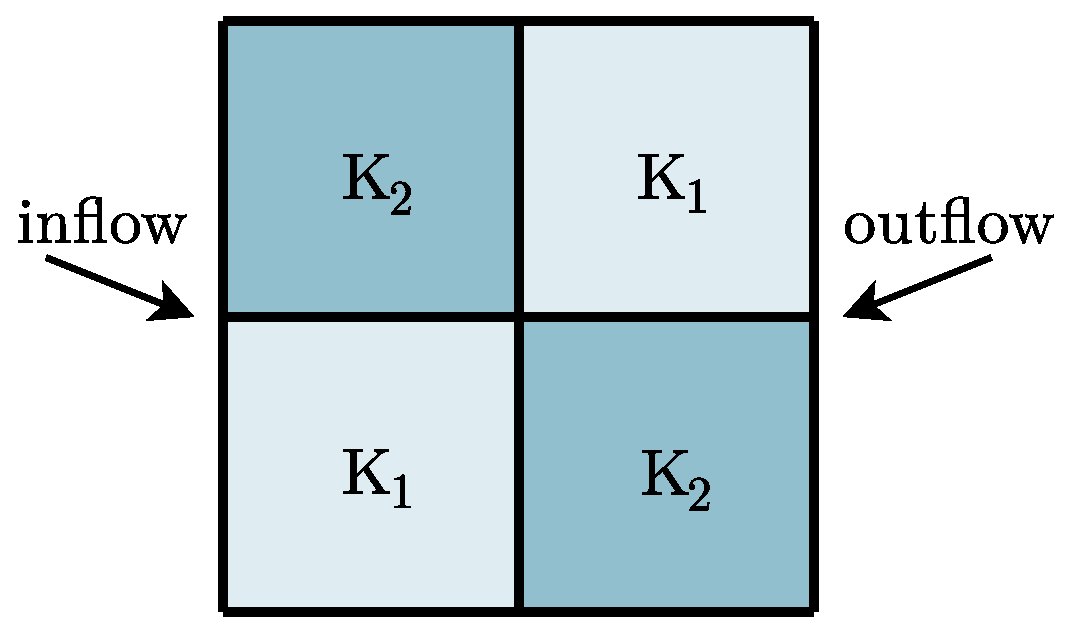
\includegraphics[width=0.5\textwidth]{4Rregion_BLv2}
    \caption{Schematic of the computational domain along with the
      material properties and boundary conditions for the
      heterogeneous permeability test case. Darker areas
      ($\mathbf{K}_\text{1}$) represent regions with high
      permeability. \label{fig:4reg_BL_schematic}}
  \end{center}
\end{figure}

\begin{figure}[h!]
  \centering
  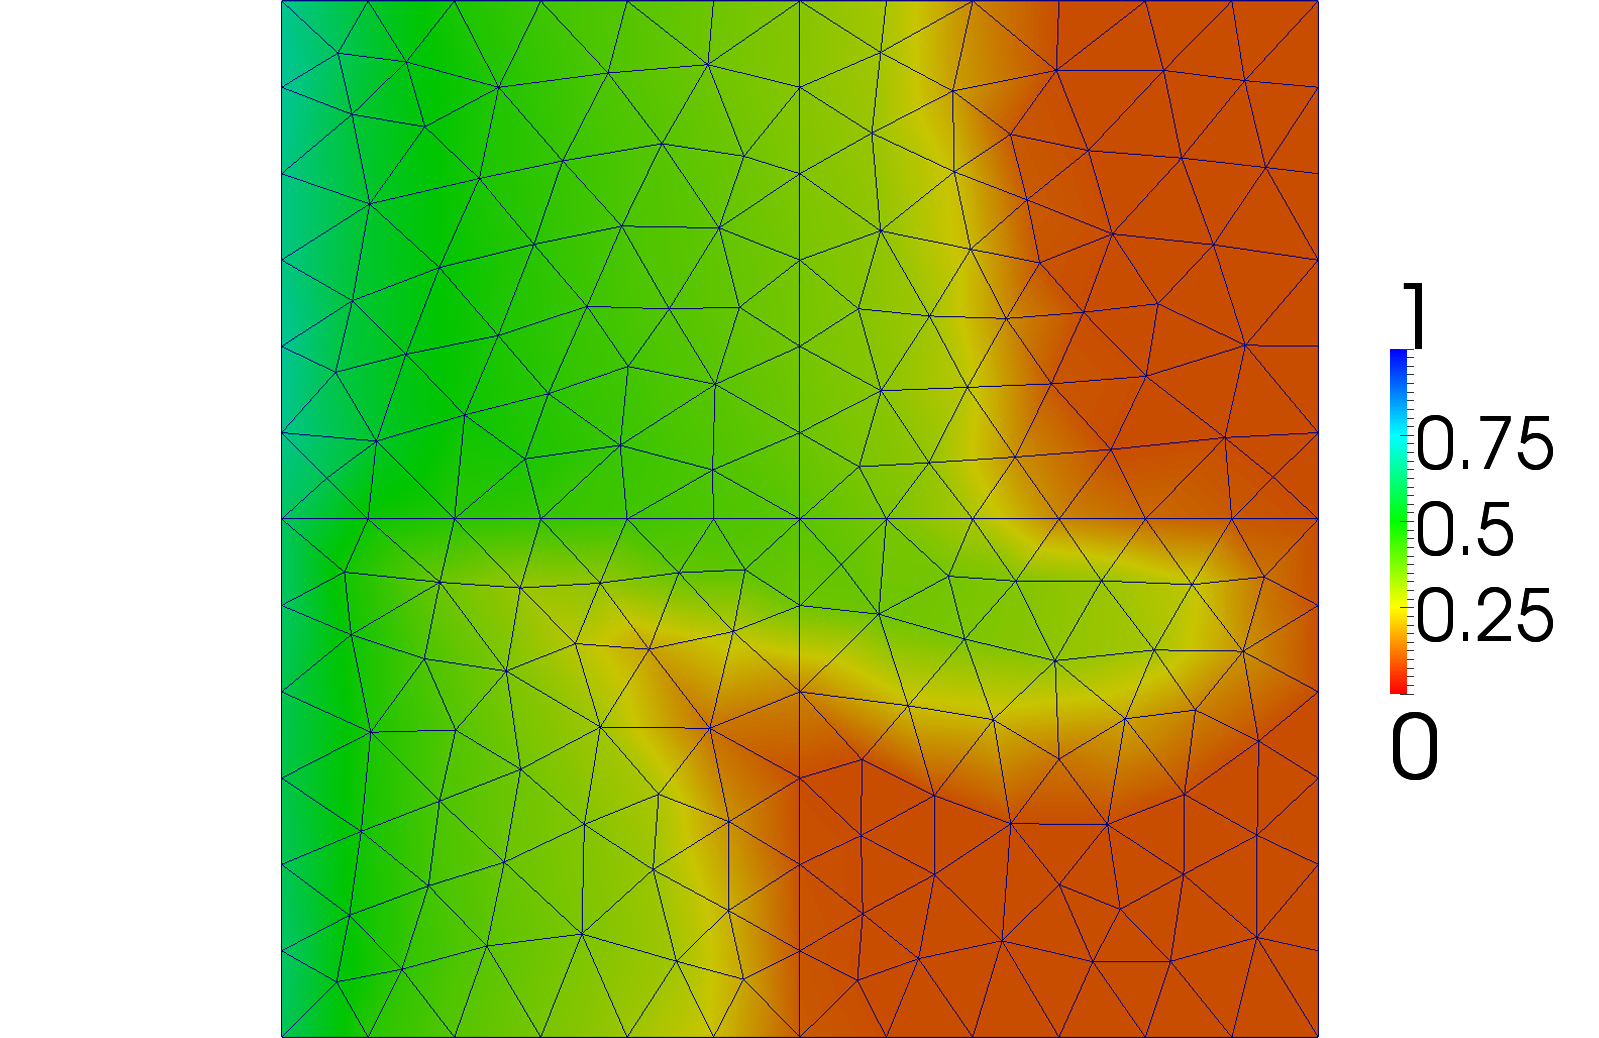
\includegraphics[width=0.45\textwidth]{CG_coarse083.png}
  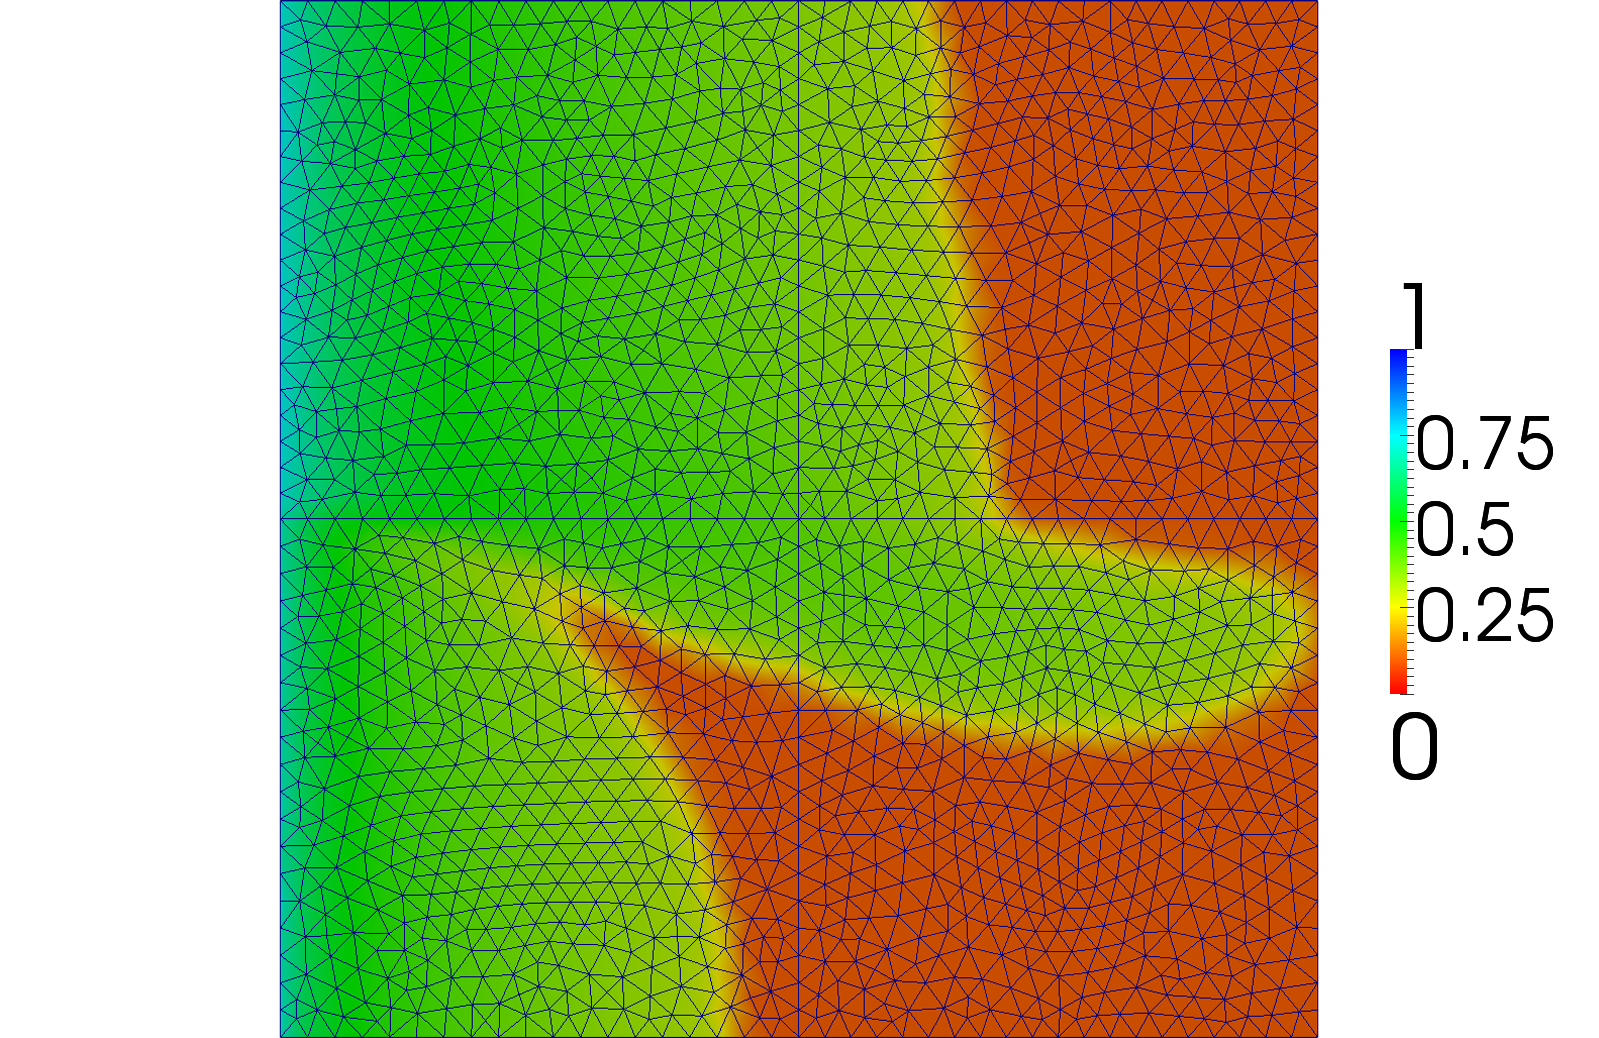
\includegraphics[width=0.45\textwidth]{CG_fine083.png}
  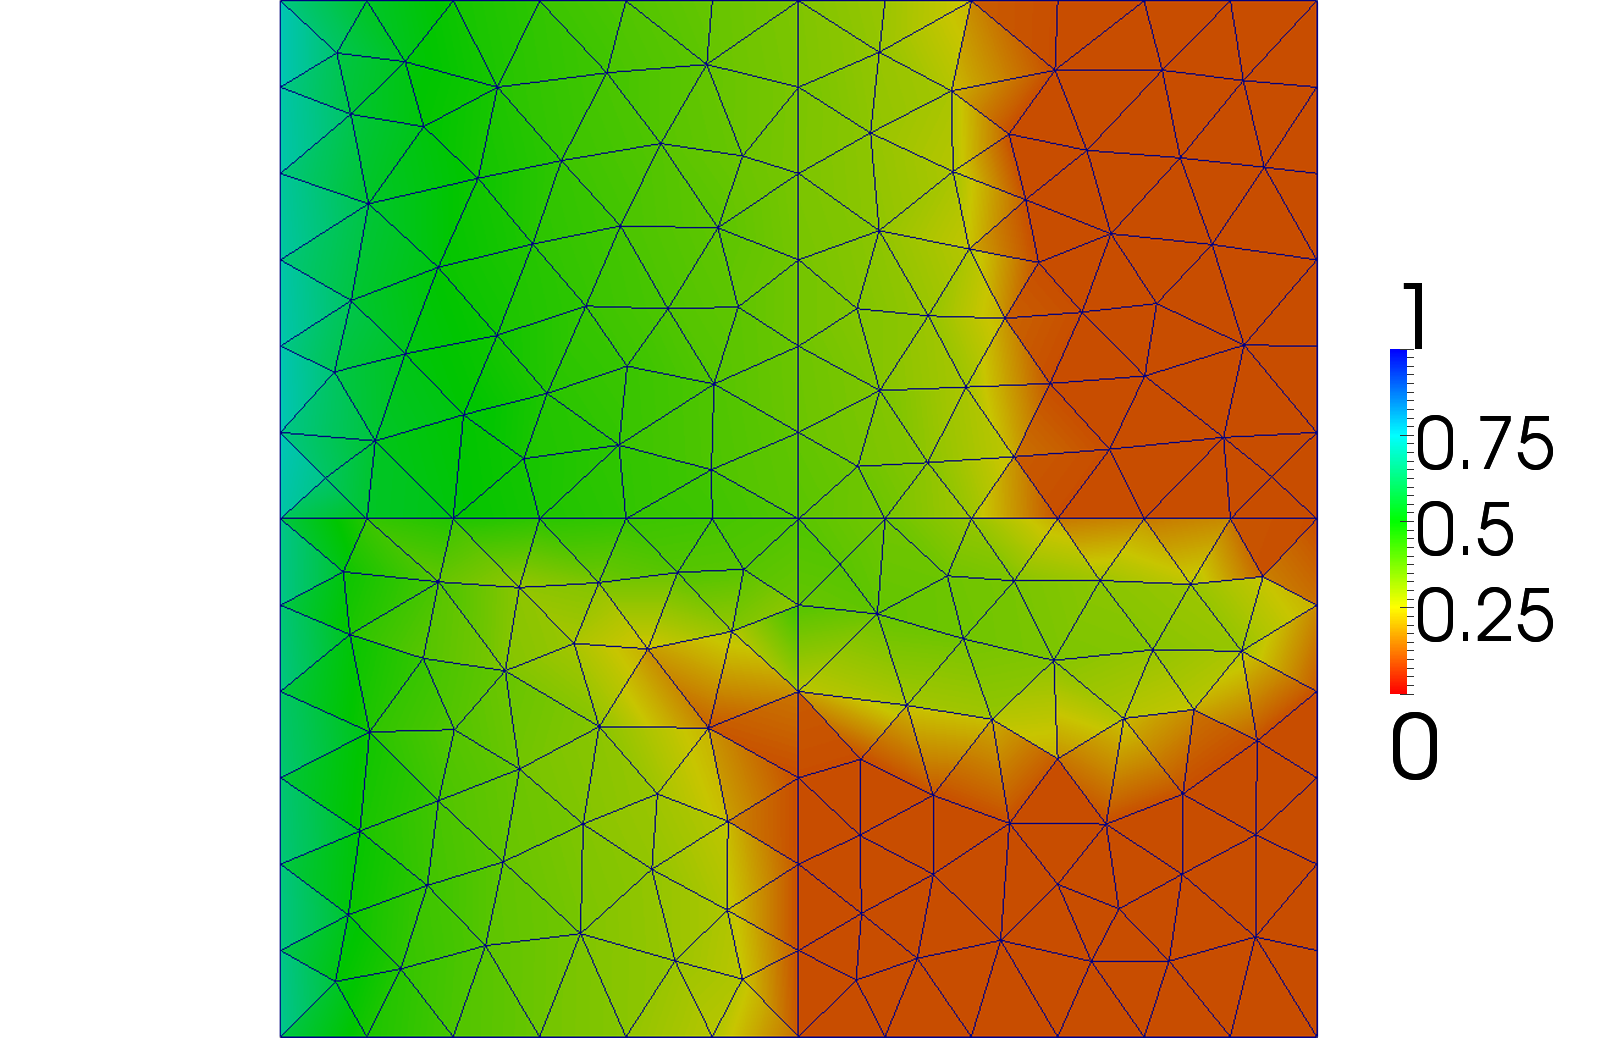
\includegraphics[width=0.45\textwidth]{DG_coarse083.png}
  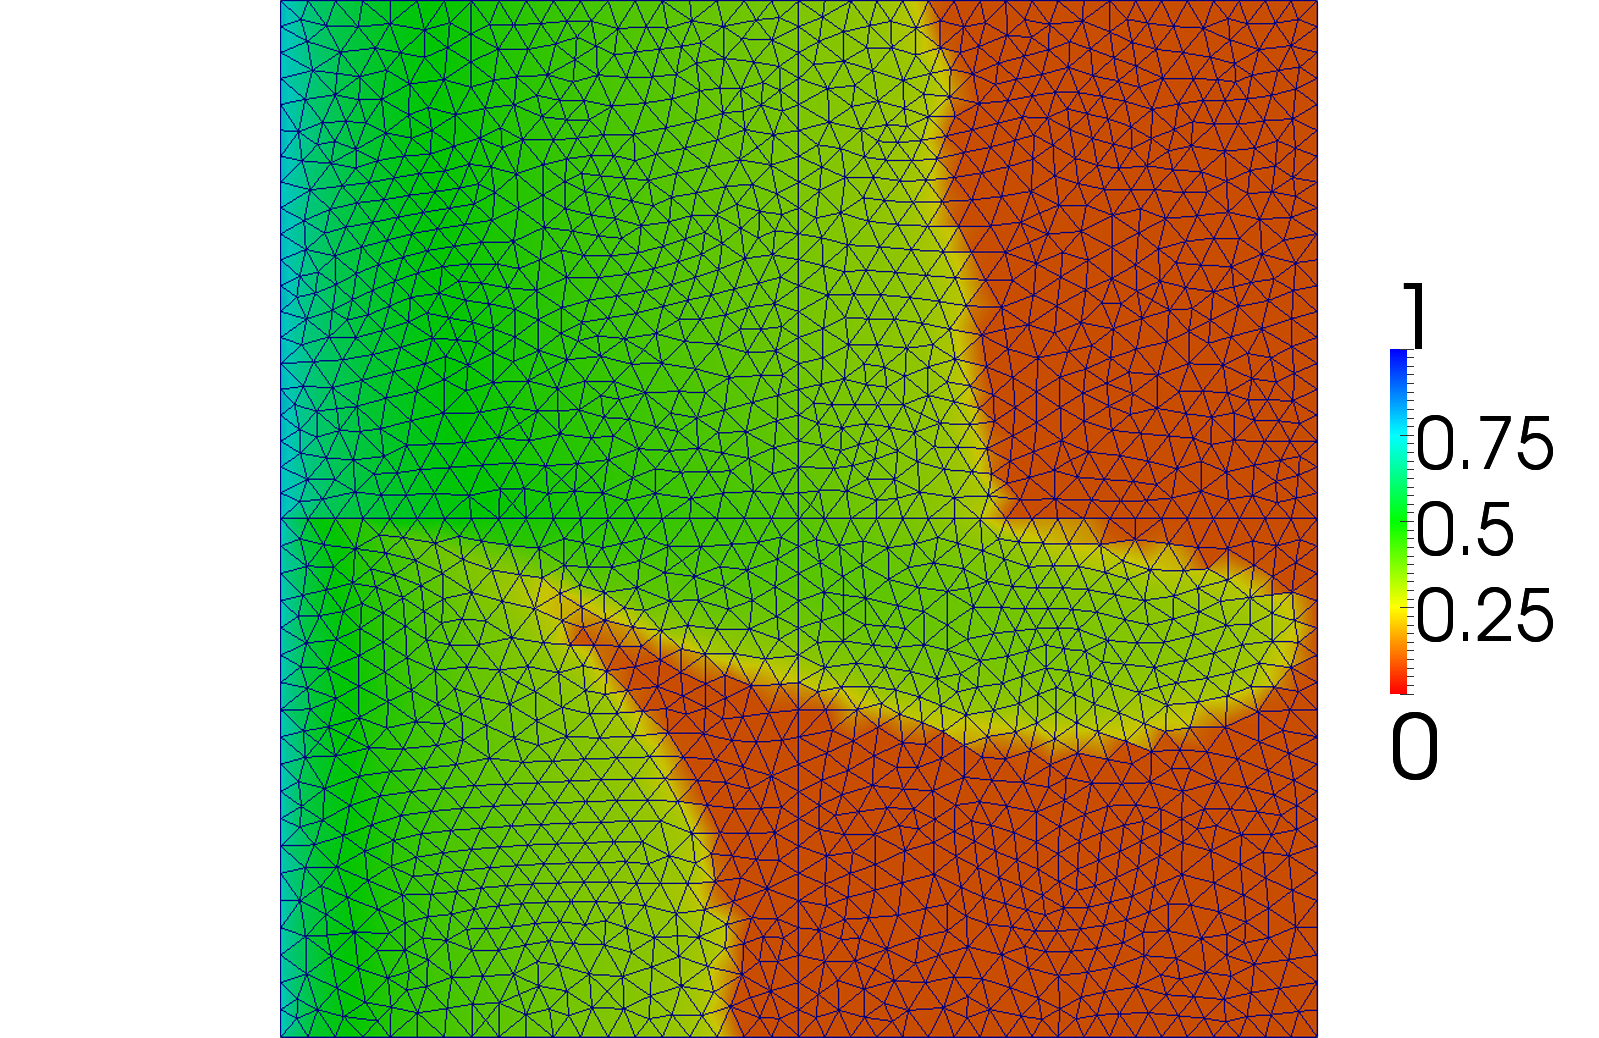
\includegraphics[width=0.45\textwidth]{DG_fine083.png}
  \caption{Wetting phase volume fraction maps at time $t=0.16$ for the
    heterogeneous permeability test case. Top row: \PN[1]{2}
    elements. Bottom row: \PN[2]{1}DG elements. Left column: coarse
    mesh. Right column: fine mesh. \label{fig:4reg_maps}}%The meshes used for these simulations are also shown here.\label{fig:4reg_maps}}
\end{figure}

\begin{figure}[h!]
  \begin{center}
    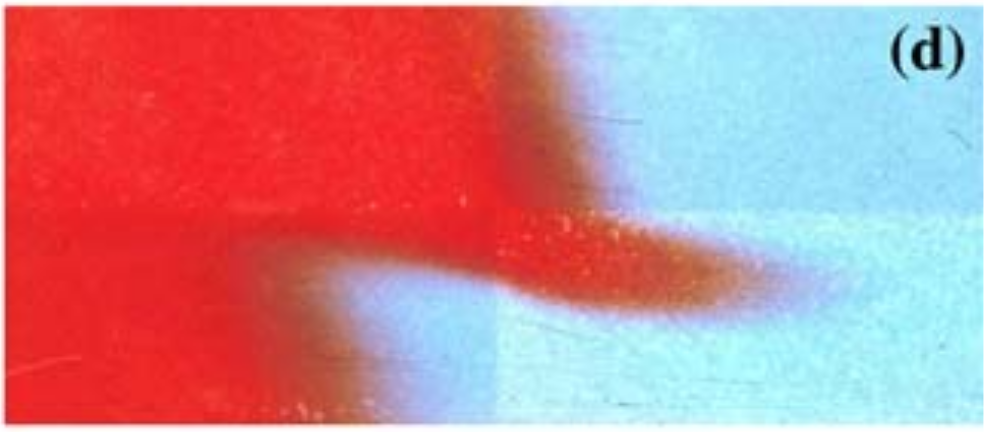
\includegraphics[width=0.6\textwidth]{Real_quadrant}
    \caption{Wetting phase volume fraction map obtained from the experiment performed by Dawe and Grattoni (extracted from \cite{dawe_2008}). Red contour indicates the injected fluid breakthrough. Geometry and permeability distribution used in this experiment is the same as shown in Fig.~\ref{fig:4reg_BL_schematic}. \label{fig:dawe_real}}
  \end{center}
\end{figure}

Two sets of simulations are performed using coarse (402 elements) and
fine (3714 elements) meshes; in the first set the \PN[1]{2} element
pair is used, while in the second one the \PN[2]{1}DG element pair is
used. The time step sizes for the coarse and fine mesh simulations are
5$\times$10$^{-3}$ and 10$^{-3}$ non-dimensional time units,
respectively.

Figure~\ref{fig:4reg_maps} shows the wetting phase volume fraction maps
at time $t=0.16$ for all four simulations. Results for the
\PN[1]{2} element pair set of simulations is shown in the top row.
Results for the \PN[2]{1}DG element pair set of simulations is shown
in the bottom row.

A physical experiment with similar set-up was performed by Dawe and Grattoni
\cite{dawe_2008} to investigate miscible and immiscible displacement
in heterogeneous permeability and wettability cases. For immiscible
displacement, the wetting phase was uniformly injected at rate of
$\approx 1$ml/min in a domain of 20cm$\times$10cm$\times$0.6cm. Glass
ballotini beads produced porosity of 0.4. The permeability ratio was
2.5.

Snapshots in Fig.~\ref{fig:4reg_maps} show the wetting phase flood
`fingering' across the four region intersection, demonstrating the
preferential flow through high permeability regions. This is in good
qualitative agreement with the experimental results
(see Fig.~\ref{fig:dawe_real}, taken from Dawe and Grattoni \cite{dawe_2008}).

\subsection{High permeability high aspect ratio region}\label{res4}

Fractures and cracks in porous media are ubiquitous, however, they are
not easy to model due to their high aspect ratio and small size
compared to the reservoir domain. Nonetheless, cracks may have a
dramatic impact in the overall behaviour of the flow as they can
channelise the flow through them. Usually, they are characterised by a
thin tip and a high permeability. A simplified 2D wedge-shaped
high permeability region embedded in a rectangular low-permeability
domain is considered here. The permeability map is shown in
Fig.~\ref{fig:wedge_permeability}. The wedge aspect ratio is $1/30$
and its maximum height is 0.025.

\begin{figure}[h!]
  \vbox{
    \hbox{
      \hspace{-0.cm}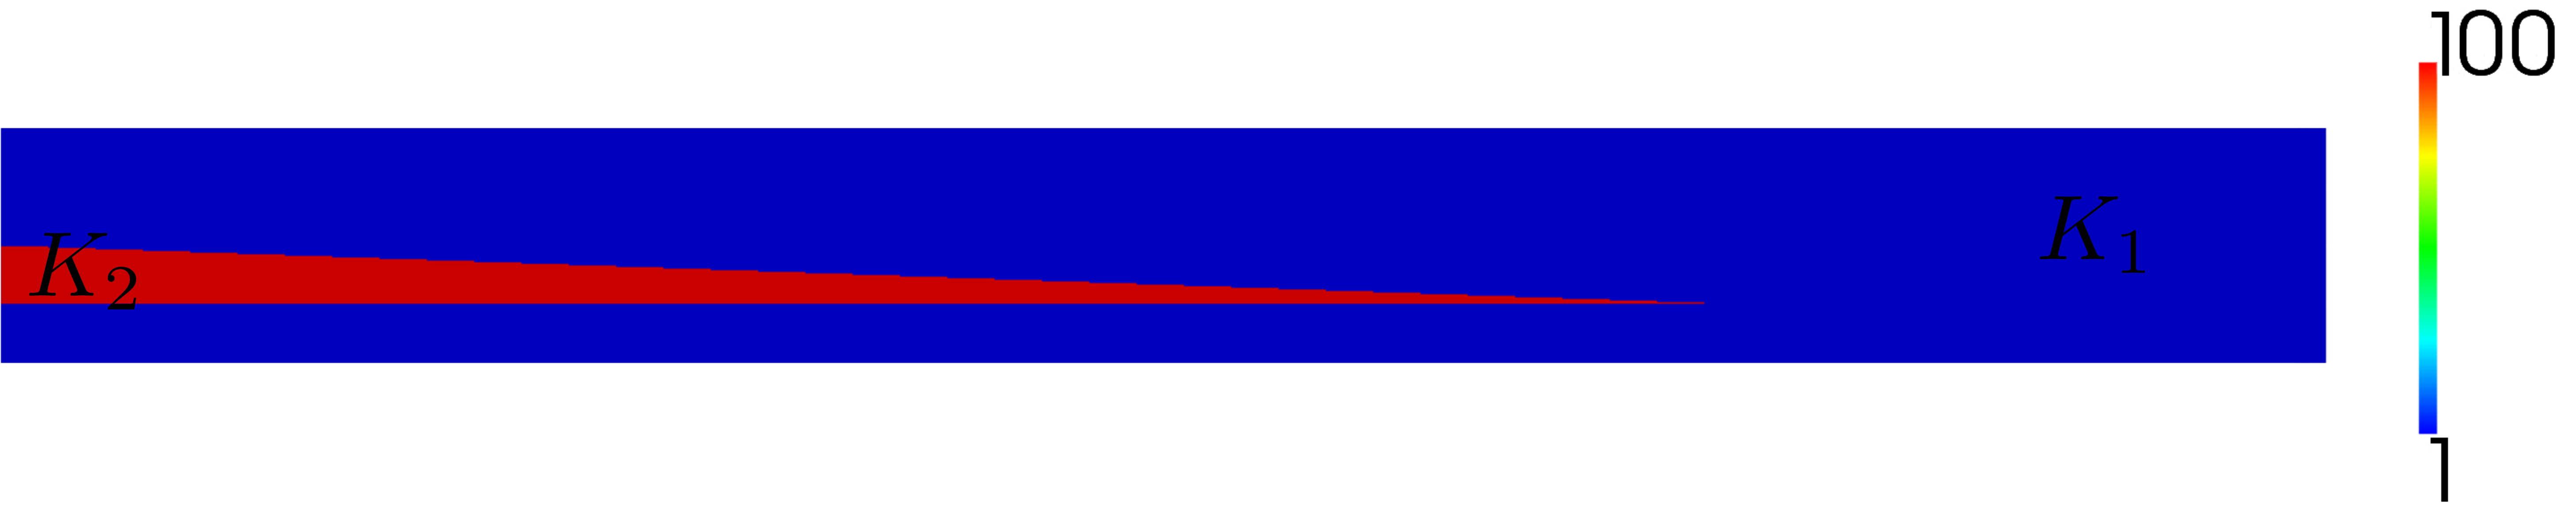
\includegraphics[width=1.0\textwidth]{wedge_permeabilityv2}}
    \vspace{-1.cm}\hbox{\hspace{4cm}(a)}
    \vspace{.5cm}
    \hbox{
      \hspace{-0.cm}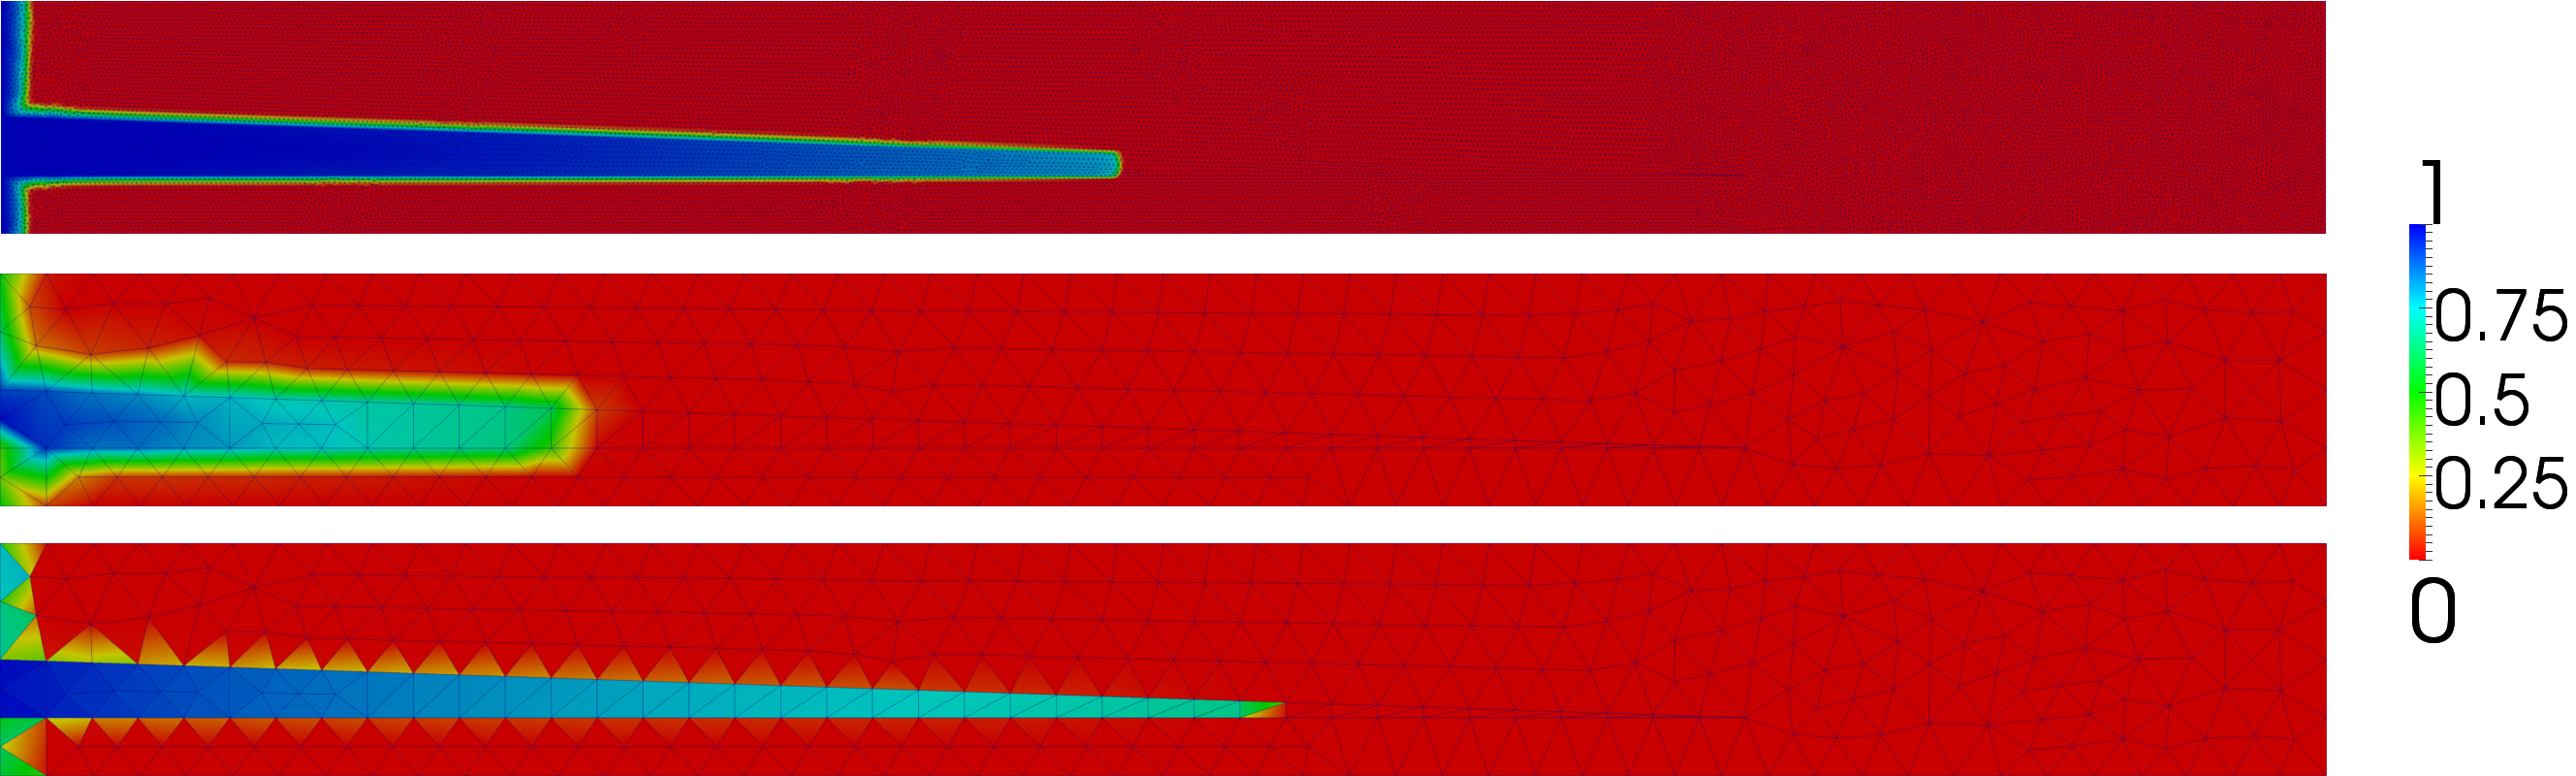
\includegraphics[width=1.0\textwidth]{wedge_0011}}
    \vspace{-0.cm}\hbox{\hspace{4cm}(b)}
    \vspace{.5cm}
    \hbox{
      \hspace{-.cm}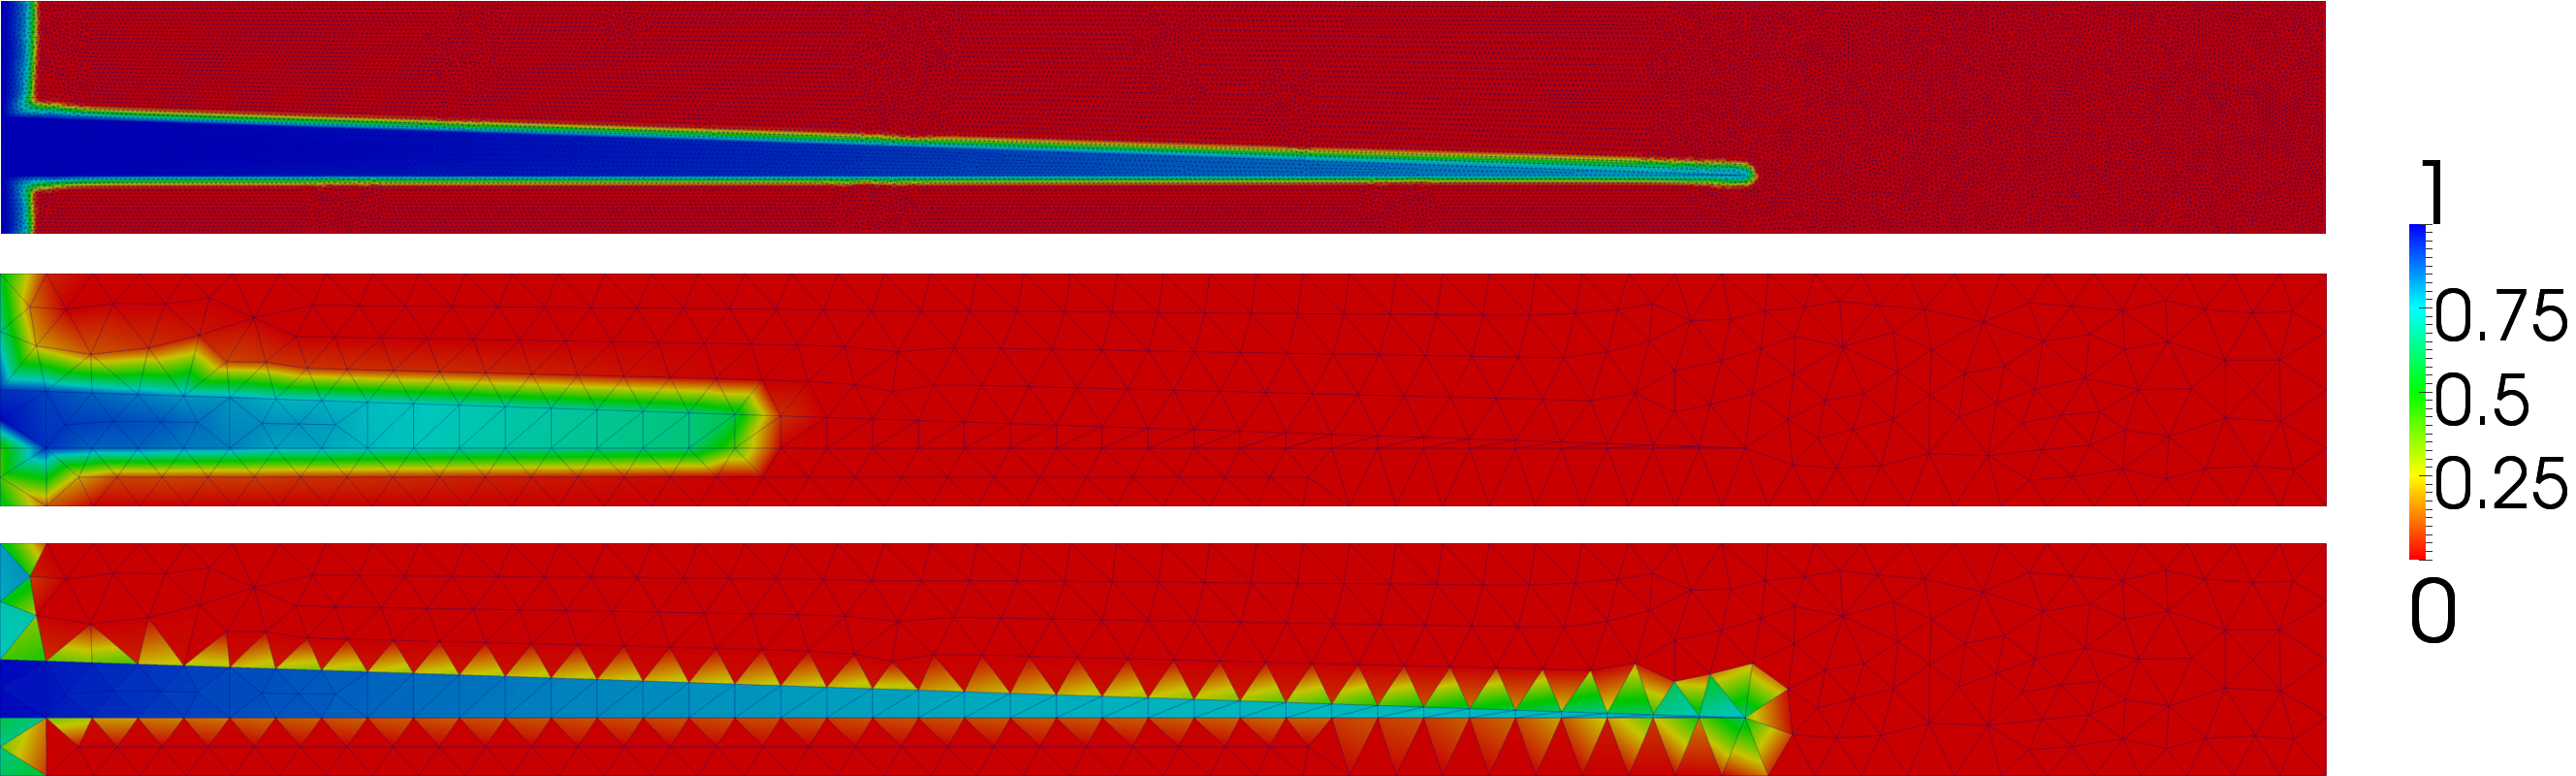
\includegraphics[width=1.0\textwidth]{wedge_0014}}
    \vspace{-0.cm}\hbox{\hspace{4cm}(c)}
  }
  \caption{Schematic of the computational domain along with the
    permeability map for the high permeability wedge-shaped region
    test case (a). Snapshots of the wetting phase volume fraction
    field for a fine mesh \PN[1]{2} simulation (top), coarse mesh
    \PN[1]{2} simulation (middle) and coarse mesh \PN[2]{1}DG
    simulation (bottom) at non-dimensional times $t = 0.011$ (b) and
    $t=0.0014$ (c). The meshes used for these simulations are also
    shown in (b) and (c).
    \label{fig:wedge_permeability}}
\end{figure}

Three numerical simulations are performed in total. Two use the
\PN[1]{2} element pair and one uses the \PN[2]{1}DG element pair.
\PN[1]{2} element pair simulations are performed using a coarse (672
elements) and a fine (56902 elements) mesh. The coarse mesh is used
for the \PN[2]{1}DG element pair simulation.

Fig.~\ref{fig:wedge_permeability} shows wetting phase volume fraction
maps at non-dimensional times $t=0.011$ and 0.014. The \PN[1]{2}-based
solutions disperse the wetting phase into the low-permeability
matrix. This is more pronounced for the coarse mesh simulation. It can
be seen how the front of the wetting phase is considerably delayed
compared with the other two simulations. On the other hand, the
\PN[2]{1}DG solution does not disperse the wetting phase into the
matrix and even a very coarse mesh is sufficient to accurately capture
the flow.

\subsection{3D fluvial channel model}\label{res5}

\begin{figure}[h!]
  \vbox{
    \hbox{
      \hspace{3.5cm} 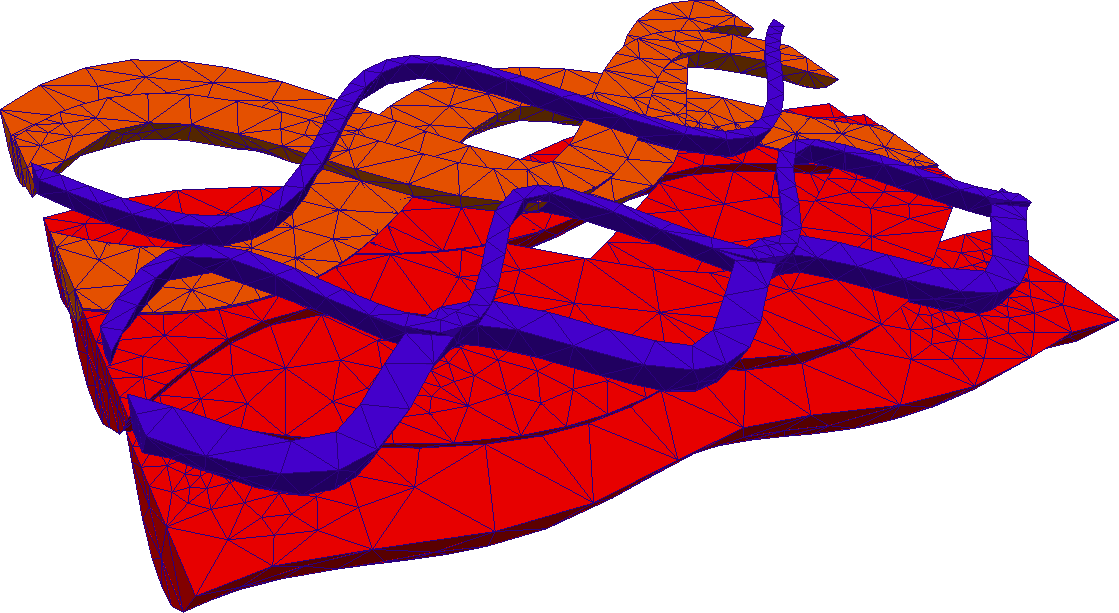
\includegraphics[width=0.45\textwidth]{permeability_map}}
    \vspace{0.1cm}
    \hbox{
      \hspace{0.0cm}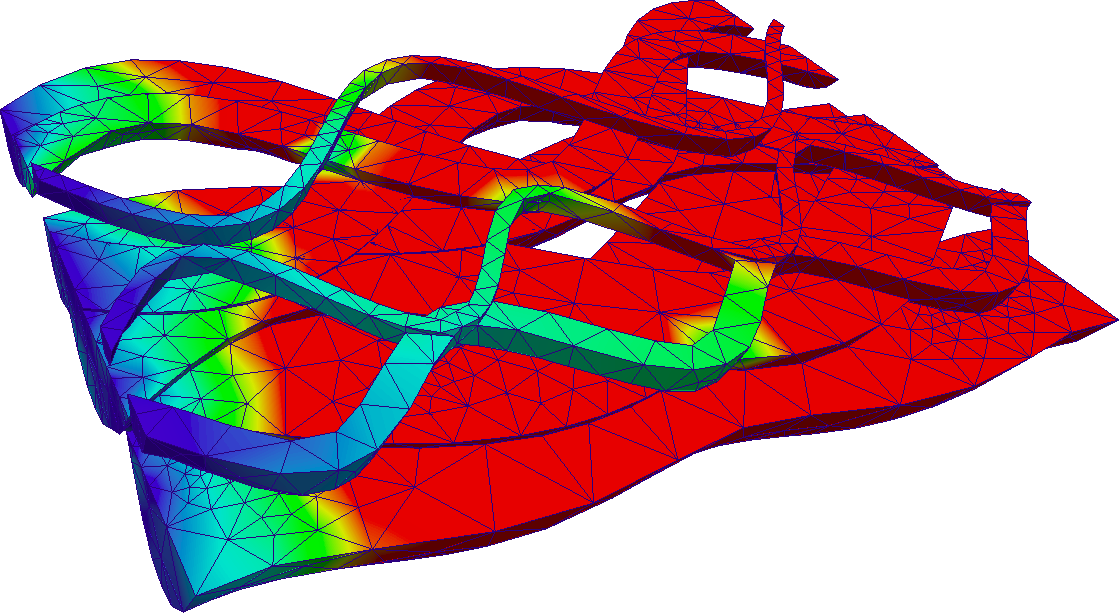
\includegraphics[width=0.475\textwidth]{phase_vol_fraction_vtu10}
      \hspace{0.0cm}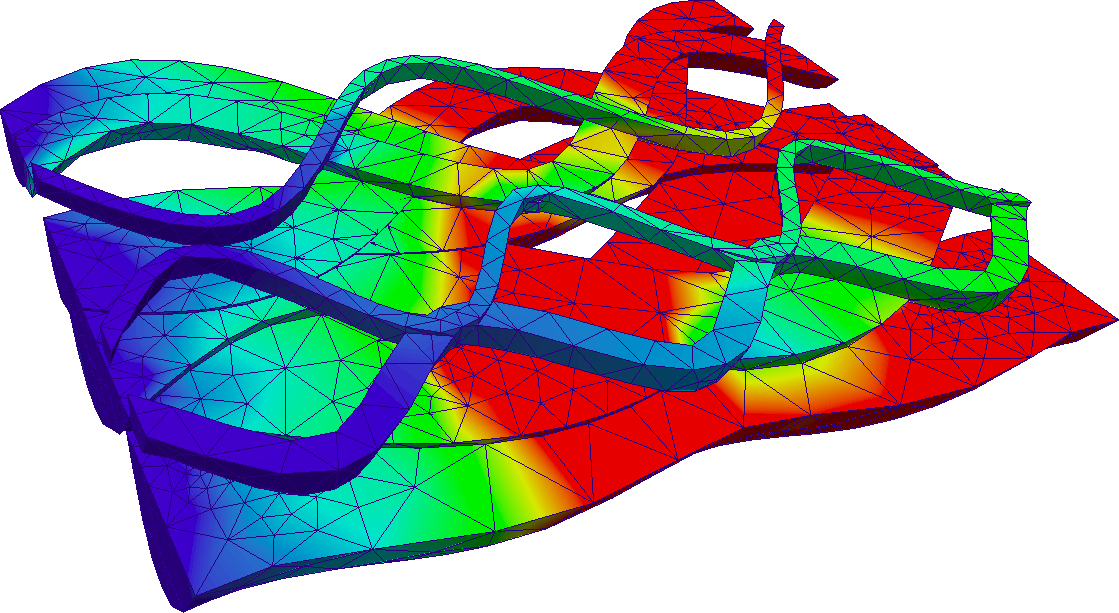
\includegraphics[width=0.475\textwidth]{phase_vol_fraction_vtu20}}
    \vspace{0.1cm}
    \hbox{
      \hspace{0.0cm}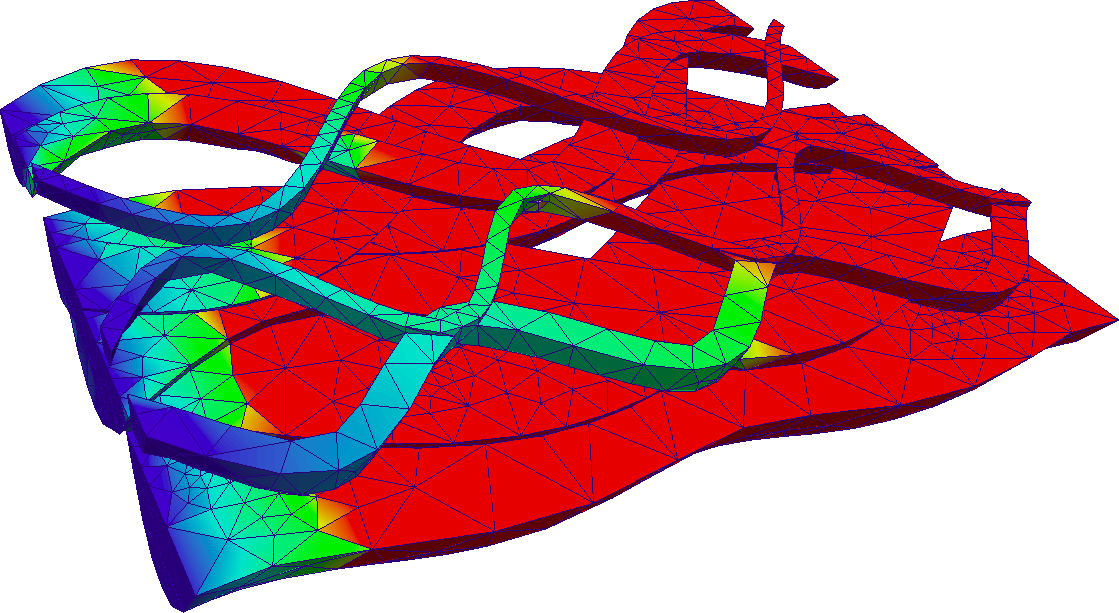
\includegraphics[width=0.475\textwidth]{phase_vol_fraction_DGvtu10}
      \hspace{0.0cm}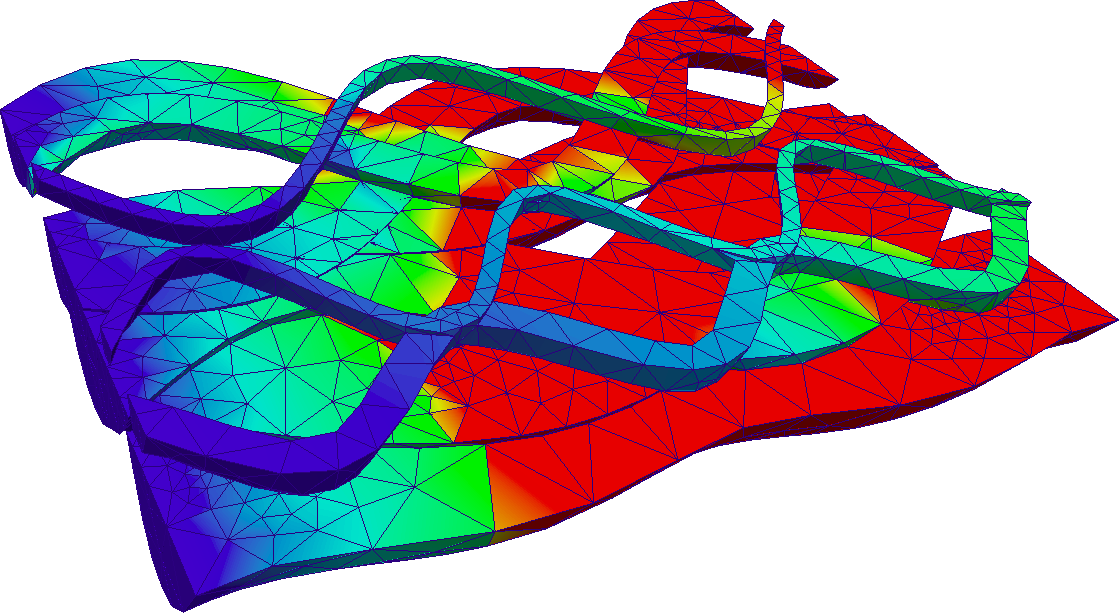
\includegraphics[width=0.475\textwidth]{phase_vol_fraction_DGvtu20}}}
  \caption{Schematic of the computational domain along with the
    permeability map and mesh used for the 3D fluvial channel case
    (top). Wetting phase volume fraction maps at two time levels
    (left and right). \PN[1]{1} element pair results are shown in the
    middle row. \PN[2]{1}DG element pair results are shown in the
    bottom row.
    \label{fig:fluvial_model}}
\end{figure}

The method is finally applied to a subsurface example of high
permeability fluvial sandstone channels embedded in a low permeability
mudstone background. Such features are often observed in aquifers and
petroleum reservoirs. Due to the importance of these channels to the
flow behaviour, their correct representation and resolution is key to
obtain reliable productivity solutions. In this model three different sets of
highly permeable channels are considered. The mesh and permeability
map for these simulations are shown in Fig.~\ref{fig:fluvial_model}
(top). The thin channels have a permeability of $\mathbf{K}_\text{3}$,
the medium size channels $\mathbf{K}_\text{2}$ and the wide channels
$\mathbf{K}_\text{1}$. \red{Maybe it is worth commenting either $\mathbf{K}$ ratio or which one is the more or less permeable, i.e., $\mathbf{K}_{1} < \mathbf{K}_{2} < \mathbf{K}_{3}$ -- See reviewers' comments 4, 14 and 3.}

Two numerical simulations are performed using an 8000-element fully
unstructured mesh. Wetting phase volume fraction maps at two time
levels are shown in Fig.~\ref{fig:fluvial_model}. Results for
the \PN[1]{1}DG element pair are shown in the middle, while results
for the \PN[2]{1}DG element pair are shown in the bottom row. Results
are in reasonable agreement. It is worth noting that the \PN[1]{1}
element pair (closest to traditional CVFEM formulation) is numerically
more dispersive \red{(do we have any proof of this? either for this paper or other published paper)}. Nevertheless, these results demonstrate the potential
of the methods presented here to simulate real-world geometries.



\section{Conclusions}\label{conc}

A novel CVFEM formulation based on \PN[n]{m}(DG) element pairs with $n^{\rm th}$-order representation for velocity and $m^{\rm th}$-order for pressure has been presented. The main advantages of this formulation over existing ones is that arbitrarily high-order polynomial representation for pressure and velocity can be used and it is high-order accurate in space and time. In \PN[n]{n+1} element pairs, velocity is discontinuously defined by polynomials of order $n$ whereas pressure is continuously represented by polynomials of order $n+1$ with CVs spanning various neighbours elements, as exemplified by Fig.~\ref{fem_cv_represent_a}a. However, in the novel \PNDG[n+1]{n} element pair, introduced in this paper, both pressure and velocity have discontinuous representation with polynomials of order $n$ and $n+1$, respectively. In this family of element pairs, CVs do not span elements (see Fig.~\ref{fem_cv_represent_a}b), which resolves a long-standing problem associated with the use of traditional CVFEM formulations in heterogeneous porous media flows.

The new formulation was evaluated using the Buckley-Leverett benchmark
and first-order convergence rates were achieved for solutions with
discontinuities, which are not common in the literature
(see \cite{Schmid,Hoteit}). Second-order convergence rates were
achieved for solutions without a discontinuity. More numerical
simulations were performed to demonstrate the capabilities of the
methods presented under heterogeneous and high aspect ratio
computational domains. It was shown that the method is able to 
successfully resolve multi-phase flows under those circumstances. Furthermore,
the \PN[n+1]{n}DG element pair was shown to completely remove
numerical dispersion induced by heterogeneous permeabilities.

The formulation presented here was implemented in the open-source
software framework
\href{http://www3.imperial.ac.uk/earthscienceandengineering/research/amcg/fluidity}{Fluidity}
for multi-phase flows (IC-Ferst) and it has been extended to
include/model multi-component/interface-capturing flows
\cite{pavlidis_2013b,pavlidis_2014,xie_2014}, segregation in granular
flows \cite{percival_2014} and oil reservoir flows
\cite{jackson_2015,mostaghimi_2015, Salinas}.



\ack Dr D. Pavlidis would like to acknowledge the support from the
following research grants: Innovate UK `Octopus', EPSRC `Reactor
Core-Structure Re-location Modelling for Severe Nuclear Accidents')
and Horizon 2020 `In-Vessel Melt Retention'. Funding for Dr P. Salinas
from ExxonMobil is gratefully acknowledged. Dr Z. Xie is supported by
EPSRC `Multi-Scale Exploration of Multiphase Physics in Flows'. Part
funding for Prof Jackson under the TOTAL Chairs programme at Imperial
College is also acknowledged. The authors would also like to acknowledge
Mr Y. Debbabi for supplying analytic solutions.



\bibliographystyle{wileyj}
\bibliography{references}


\end{document}

%%
%% End of tex file.
